\documentclass[twoside]{book}

% Packages required by doxygen
\usepackage{calc}
\usepackage{doxygen}
\usepackage{graphicx}
\usepackage[utf8]{inputenc}
\usepackage{makeidx}
\usepackage{multicol}
\usepackage{multirow}
\usepackage{textcomp}
\usepackage[table]{xcolor}

% Font selection
\usepackage[T1]{fontenc}
\usepackage{mathptmx}
\usepackage[scaled=.90]{helvet}
\usepackage{courier}
\usepackage{amssymb}
\usepackage{sectsty}
\renewcommand{\familydefault}{\sfdefault}
\allsectionsfont{%
  \fontseries{bc}\selectfont%
  \color{darkgray}%
}
\renewcommand{\DoxyLabelFont}{%
  \fontseries{bc}\selectfont%
  \color{darkgray}%
}

% Page & text layout
\usepackage{geometry}
\geometry{%
  a4paper,%
  top=2.5cm,%
  bottom=2.5cm,%
  left=2.5cm,%
  right=2.5cm%
}
\tolerance=750
\hfuzz=15pt
\hbadness=750
\setlength{\emergencystretch}{15pt}
\setlength{\parindent}{0cm}
\setlength{\parskip}{0.2cm}
\makeatletter
\renewcommand{\paragraph}{%
  \@startsection{paragraph}{4}{0ex}{-1.0ex}{1.0ex}{%
    \normalfont\normalsize\bfseries\SS@parafont%
  }%
}
\renewcommand{\subparagraph}{%
  \@startsection{subparagraph}{5}{0ex}{-1.0ex}{1.0ex}{%
    \normalfont\normalsize\bfseries\SS@subparafont%
  }%
}
\makeatother

% Headers & footers
\usepackage{fancyhdr}
\pagestyle{fancyplain}
\fancyhead[LE]{\fancyplain{}{\bfseries\thepage}}
\fancyhead[CE]{\fancyplain{}{}}
\fancyhead[RE]{\fancyplain{}{\bfseries\leftmark}}
\fancyhead[LO]{\fancyplain{}{\bfseries\rightmark}}
\fancyhead[CO]{\fancyplain{}{}}
\fancyhead[RO]{\fancyplain{}{\bfseries\thepage}}
\fancyfoot[LE]{\fancyplain{}{}}
\fancyfoot[CE]{\fancyplain{}{}}
\fancyfoot[RE]{\fancyplain{}{\bfseries\scriptsize Generated on Sat Nov 9 2019 12\-:36\-:37 for My Project by Doxygen }}
\fancyfoot[LO]{\fancyplain{}{\bfseries\scriptsize Generated on Sat Nov 9 2019 12\-:36\-:37 for My Project by Doxygen }}
\fancyfoot[CO]{\fancyplain{}{}}
\fancyfoot[RO]{\fancyplain{}{}}
\renewcommand{\footrulewidth}{0.4pt}
\renewcommand{\chaptermark}[1]{%
  \markboth{#1}{}%
}
\renewcommand{\sectionmark}[1]{%
  \markright{\thesection\ #1}%
}

% Indices & bibliography
\usepackage{natbib}
\usepackage[titles]{tocloft}
\setcounter{tocdepth}{3}
\setcounter{secnumdepth}{5}
\makeindex

% Hyperlinks (required, but should be loaded last)
\usepackage{ifpdf}
\ifpdf
  \usepackage[pdftex,pagebackref=true]{hyperref}
\else
  \usepackage[ps2pdf,pagebackref=true]{hyperref}
\fi
\hypersetup{%
  colorlinks=true,%
  linkcolor=blue,%
  citecolor=blue,%
  unicode%
}

% Custom commands
\newcommand{\clearemptydoublepage}{%
  \newpage{\pagestyle{empty}\cleardoublepage}%
}


%===== C O N T E N T S =====

\begin{document}

% Titlepage & ToC
\hypersetup{pageanchor=false}
\pagenumbering{roman}
\begin{titlepage}
\vspace*{7cm}
\begin{center}%
{\Large My Project }\\
\vspace*{1cm}
{\large Generated by Doxygen 1.8.6}\\
\vspace*{0.5cm}
{\small Sat Nov 9 2019 12:36:37}\\
\end{center}
\end{titlepage}
\clearemptydoublepage
\tableofcontents
\clearemptydoublepage
\pagenumbering{arabic}
\hypersetup{pageanchor=true}

%--- Begin generated contents ---
\chapter{Phase 2 Submission}
\label{index}\hypertarget{index}{}\begin{DoxyAuthor}{Author}
Mehieddine Zeidan 

Hadi Sandid 
\end{DoxyAuthor}
\begin{DoxyDate}{Date}
9-\/10-\/2019 
\end{DoxyDate}

\chapter{Hierarchical Index}
\section{Class Hierarchy}
This inheritance list is sorted roughly, but not completely, alphabetically\-:\begin{DoxyCompactList}
\item Q\-Graphics\-Pixmap\-Item\begin{DoxyCompactList}
\item \contentsline{section}{game\-Scene\-\_\-1\-\_\-dice}{\pageref{classgameScene__1__dice}}{}
\item \contentsline{section}{gamescene\-\_\-1\-\_\-ladder\-Snake}{\pageref{classgamescene__1__ladderSnake}}{}
\item \contentsline{section}{game\-Scene\-\_\-1\-\_\-player}{\pageref{classgameScene__1__player}}{}
\end{DoxyCompactList}
\item Q\-Graphics\-Scene\begin{DoxyCompactList}
\item \contentsline{section}{game\-Scene\-\_\-1}{\pageref{classgameScene__1}}{}
\end{DoxyCompactList}
\item Q\-Object\begin{DoxyCompactList}
\item \contentsline{section}{game\-Scene\-\_\-1\-\_\-dice}{\pageref{classgameScene__1__dice}}{}
\item \contentsline{section}{gamescene\-\_\-1\-\_\-ladder\-Snake}{\pageref{classgamescene__1__ladderSnake}}{}
\item \contentsline{section}{game\-Scene\-\_\-1\-\_\-player}{\pageref{classgameScene__1__player}}{}
\end{DoxyCompactList}
\item Q\-Widget\begin{DoxyCompactList}
\item \contentsline{section}{birthdaywidget}{\pageref{classbirthdaywidget}}{}
\item \contentsline{section}{login\-Widget}{\pageref{classloginWidget}}{}
\item \contentsline{section}{menu\-Widget}{\pageref{classmenuWidget}}{}
\item \contentsline{section}{register\-Widget}{\pageref{classregisterWidget}}{}
\end{DoxyCompactList}
\end{DoxyCompactList}

\chapter{Class Index}
\section{Class List}
Here are the classes, structs, unions and interfaces with brief descriptions\-:\begin{DoxyCompactList}
\item\contentsline{section}{\hyperlink{classbirthdaywidget}{birthdaywidget} }{\pageref{classbirthdaywidget}}{}
\item\contentsline{section}{\hyperlink{classgameScene__1}{game\-Scene\-\_\-1} }{\pageref{classgameScene__1}}{}
\item\contentsline{section}{\hyperlink{classgameScene__1__dice}{game\-Scene\-\_\-1\-\_\-dice} }{\pageref{classgameScene__1__dice}}{}
\item\contentsline{section}{\hyperlink{classgamescene__1__ladderSnake}{gamescene\-\_\-1\-\_\-ladder\-Snake} }{\pageref{classgamescene__1__ladderSnake}}{}
\item\contentsline{section}{\hyperlink{classgameScene__1__player}{game\-Scene\-\_\-1\-\_\-player} }{\pageref{classgameScene__1__player}}{}
\item\contentsline{section}{\hyperlink{classloginWidget}{login\-Widget} }{\pageref{classloginWidget}}{}
\item\contentsline{section}{\hyperlink{classmenuWidget}{menu\-Widget} }{\pageref{classmenuWidget}}{}
\item\contentsline{section}{\hyperlink{classregisterWidget}{register\-Widget} }{\pageref{classregisterWidget}}{}
\end{DoxyCompactList}

\chapter{File Index}
\section{File List}
Here is a list of all documented files with brief descriptions\-:\begin{DoxyCompactList}
\item\contentsline{section}{\hyperlink{birthdaywidget_8cpp}{birthdaywidget.\-cpp} \\*Contains birthdaywidget class definition }{\pageref{birthdaywidget_8cpp}}{}
\item\contentsline{section}{\hyperlink{birthdaywidget_8h}{birthdaywidget.\-h} \\*The birthdaywidget class }{\pageref{birthdaywidget_8h}}{}
\item\contentsline{section}{\hyperlink{gamescene__1_8h}{gamescene\-\_\-1.\-h} \\*The \hyperlink{classgameScene__1}{game\-Scene\-\_\-1} class }{\pageref{gamescene__1_8h}}{}
\item\contentsline{section}{\hyperlink{gamescene__1__dice_8h}{gamescene\-\_\-1\-\_\-dice.\-h} \\*The \hyperlink{classgameScene__1__dice}{game\-Scene\-\_\-1\-\_\-dice} class }{\pageref{gamescene__1__dice_8h}}{}
\item\contentsline{section}{{\bfseries gamescene\-\_\-1\-\_\-ladder\-Snake.\-h} }{\pageref{gamescene__1__ladderSnake_8h}}{}
\item\contentsline{section}{{\bfseries gamescene\-\_\-1\-\_\-player.\-h} }{\pageref{gamescene__1__player_8h}}{}
\item\contentsline{section}{{\bfseries loginwidget.\-h} }{\pageref{loginwidget_8h}}{}
\item\contentsline{section}{\hyperlink{menuwidget_8cpp}{menuwidget.\-cpp} \\*Contains \hyperlink{classmenuWidget}{menu\-Widget} class definition }{\pageref{menuwidget_8cpp}}{}
\item\contentsline{section}{\hyperlink{menuwidget_8h}{menuwidget.\-h} \\*The \hyperlink{classmenuWidget}{menu\-Widget} class }{\pageref{menuwidget_8h}}{}
\item\contentsline{section}{\hyperlink{registerwidget_8cpp}{registerwidget.\-cpp} \\*Contains \hyperlink{classregisterWidget}{register\-Widget} class definition }{\pageref{registerwidget_8cpp}}{}
\item\contentsline{section}{{\bfseries registerwidget.\-h} }{\pageref{registerwidget_8h}}{}
\end{DoxyCompactList}

\chapter{Class Documentation}
\hypertarget{classbirthdaywidget}{\section{birthdaywidget Class Reference}
\label{classbirthdaywidget}\index{birthdaywidget@{birthdaywidget}}
}
Inheritance diagram for birthdaywidget\-:\begin{figure}[H]
\begin{center}
\leavevmode
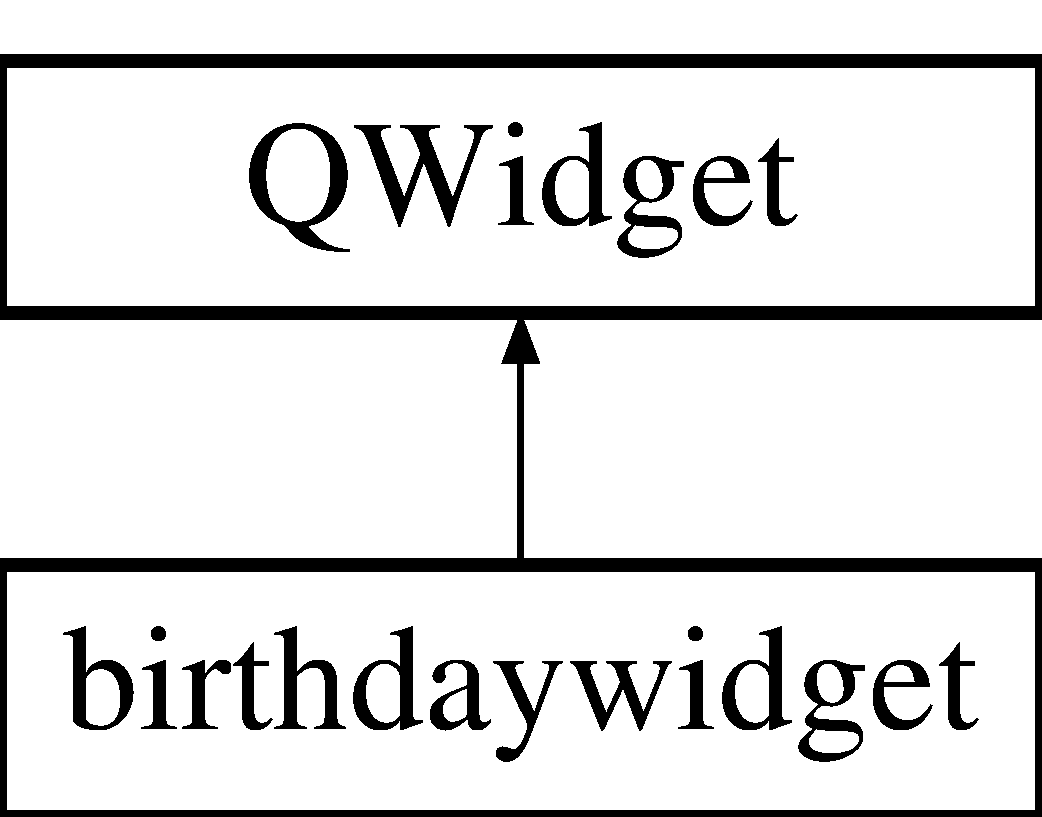
\includegraphics[height=2.000000cm]{classbirthdaywidget}
\end{center}
\end{figure}
\subsection*{Public Slots}
\begin{DoxyCompactItemize}
\item 
void \hyperlink{classbirthdaywidget_a099d4cbfc1b9bb95dd358325498832f8}{confirm\-Exit} ()
\begin{DoxyCompactList}\small\item\em \hyperlink{classbirthdaywidget_a099d4cbfc1b9bb95dd358325498832f8}{birthdaywidget\-::confirm\-Exit} \end{DoxyCompactList}\end{DoxyCompactItemize}
\subsection*{Public Member Functions}
\begin{DoxyCompactItemize}
\item 
\hypertarget{classbirthdaywidget_af8dcaa27ab4934036d0f3829c9434005}{{\bfseries birthdaywidget} (Q\-Widget $\ast$parent=0)}\label{classbirthdaywidget_af8dcaa27ab4934036d0f3829c9434005}

\end{DoxyCompactItemize}
\subsection*{Public Attributes}
\begin{DoxyCompactItemize}
\item 
\hypertarget{classbirthdaywidget_ae0305457ee51a443d68d318c68f1e687}{Q\-V\-Box\-Layout $\ast$ \hyperlink{classbirthdaywidget_ae0305457ee51a443d68d318c68f1e687}{layout}}\label{classbirthdaywidget_ae0305457ee51a443d68d318c68f1e687}

\begin{DoxyCompactList}\small\item\em V\-Box Layout. \end{DoxyCompactList}\item 
\hypertarget{classbirthdaywidget_a0b92c57cf2db67cc46e46ff95c6d822b}{Q\-Label $\ast$ \hyperlink{classbirthdaywidget_a0b92c57cf2db67cc46e46ff95c6d822b}{bdtext}}\label{classbirthdaywidget_a0b92c57cf2db67cc46e46ff95c6d822b}

\begin{DoxyCompactList}\small\item\em Main text. \end{DoxyCompactList}\item 
\hypertarget{classbirthdaywidget_a6166e41b92e8b30a4ab4a61c3ba19913}{Q\-Push\-Button $\ast$ \hyperlink{classbirthdaywidget_a6166e41b92e8b30a4ab4a61c3ba19913}{conf}}\label{classbirthdaywidget_a6166e41b92e8b30a4ab4a61c3ba19913}

\begin{DoxyCompactList}\small\item\em Main Button. \end{DoxyCompactList}\end{DoxyCompactItemize}


\subsection{Member Function Documentation}
\hypertarget{classbirthdaywidget_a099d4cbfc1b9bb95dd358325498832f8}{\index{birthdaywidget@{birthdaywidget}!confirm\-Exit@{confirm\-Exit}}
\index{confirm\-Exit@{confirm\-Exit}!birthdaywidget@{birthdaywidget}}
\subsubsection[{confirm\-Exit}]{\setlength{\rightskip}{0pt plus 5cm}void birthdaywidget\-::confirm\-Exit (
\begin{DoxyParamCaption}
{}
\end{DoxyParamCaption}
)\hspace{0.3cm}{\ttfamily [slot]}}}\label{classbirthdaywidget_a099d4cbfc1b9bb95dd358325498832f8}


\hyperlink{classbirthdaywidget_a099d4cbfc1b9bb95dd358325498832f8}{birthdaywidget\-::confirm\-Exit} 

Exit from birthday message 

The documentation for this class was generated from the following files\-:\begin{DoxyCompactItemize}
\item 
\hyperlink{birthdaywidget_8h}{birthdaywidget.\-h}\item 
\hyperlink{birthdaywidget_8cpp}{birthdaywidget.\-cpp}\end{DoxyCompactItemize}

\hypertarget{classgameScene__1}{\section{game\-Scene\-\_\-1 Class Reference}
\label{classgameScene__1}\index{game\-Scene\-\_\-1@{game\-Scene\-\_\-1}}
}
Inheritance diagram for game\-Scene\-\_\-1\-:\begin{figure}[H]
\begin{center}
\leavevmode
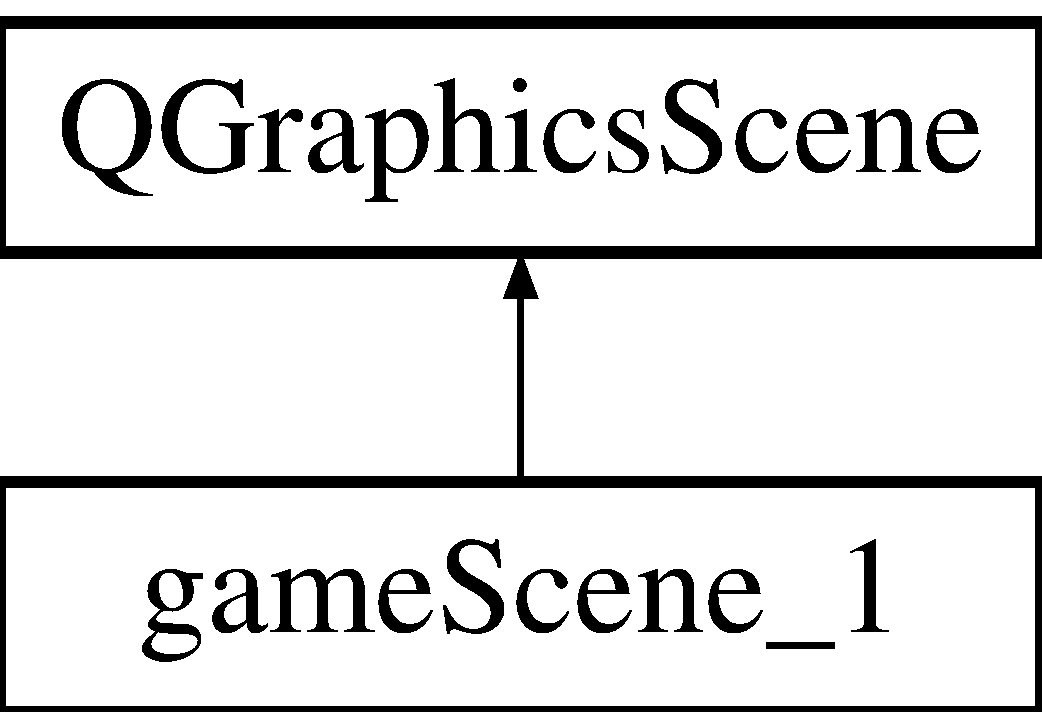
\includegraphics[height=2.000000cm]{classgameScene__1}
\end{center}
\end{figure}
\subsection*{Public Slots}
\begin{DoxyCompactItemize}
\item 
void \hyperlink{classgameScene__1_a8f81fbee2899f19fcab6f47e204843fb}{generate\-Board} ()
\begin{DoxyCompactList}\small\item\em \hyperlink{classgameScene__1_a8f81fbee2899f19fcab6f47e204843fb}{game\-Scene\-\_\-1\-::generate\-Board} \end{DoxyCompactList}\item 
void \hyperlink{classgameScene__1_a20057c5ea6cca6194aa5f5834f71687a}{select\-Left} ()
\begin{DoxyCompactList}\small\item\em \hyperlink{classgameScene__1_a20057c5ea6cca6194aa5f5834f71687a}{game\-Scene\-\_\-1\-::select\-Left} \end{DoxyCompactList}\item 
void \hyperlink{classgameScene__1_a08c914a59a8f2edc33e1cfdff0b4c06f}{select\-Right} ()
\begin{DoxyCompactList}\small\item\em \hyperlink{classgameScene__1_a08c914a59a8f2edc33e1cfdff0b4c06f}{game\-Scene\-\_\-1\-::select\-Right} \end{DoxyCompactList}\item 
void \hyperlink{classgameScene__1_ad115e2a57fa8f9927ba6e4bc22c6361d}{dice\-Roll} ()
\begin{DoxyCompactList}\small\item\em \hyperlink{classgameScene__1_ad115e2a57fa8f9927ba6e4bc22c6361d}{game\-Scene\-\_\-1\-::dice\-Roll} \end{DoxyCompactList}\item 
\hypertarget{classgameScene__1_a75c74fdbc955e234e02750b524a8523f}{void {\bfseries check\-Snake\-Ladder} ()}\label{classgameScene__1_a75c74fdbc955e234e02750b524a8523f}

\item 
void \hyperlink{classgameScene__1_a026876720e48a3afb040f8bc19ec6279}{win\-Condition} ()
\begin{DoxyCompactList}\small\item\em \hyperlink{classgameScene__1_a026876720e48a3afb040f8bc19ec6279}{game\-Scene\-\_\-1\-::win\-Condition} \end{DoxyCompactList}\item 
void \hyperlink{classgameScene__1_a815b68676c0afc94ba757fe37e42af69}{move\-Player} ()
\begin{DoxyCompactList}\small\item\em \hyperlink{classgameScene__1_a815b68676c0afc94ba757fe37e42af69}{game\-Scene\-\_\-1\-::move\-Player} \end{DoxyCompactList}\item 
void \hyperlink{classgameScene__1_a3e3e9cf17cfb4439cc2bf264b7d7ec19}{move\-Player\-Opp} ()
\begin{DoxyCompactList}\small\item\em \hyperlink{classgameScene__1_a3e3e9cf17cfb4439cc2bf264b7d7ec19}{game\-Scene\-\_\-1\-::move\-Player\-Opp} \end{DoxyCompactList}\item 
void \hyperlink{classgameScene__1_a45979d160308acb26e5cd60b00568bb4}{back\-To\-Menu} ()
\begin{DoxyCompactList}\small\item\em \hyperlink{classgameScene__1_a45979d160308acb26e5cd60b00568bb4}{game\-Scene\-\_\-1\-::back\-To\-Menu} \end{DoxyCompactList}\item 
void \hyperlink{classgameScene__1_aecddbe4488e834439b5f0313478be689}{load\-Game} (int posp1, int posp2, bool turn)
\begin{DoxyCompactList}\small\item\em \hyperlink{classgameScene__1_aecddbe4488e834439b5f0313478be689}{game\-Scene\-\_\-1\-::load\-Game} \end{DoxyCompactList}\end{DoxyCompactItemize}
\subsection*{Public Member Functions}
\begin{DoxyCompactItemize}
\item 
\hypertarget{classgameScene__1_a8a253c42464547dff6802cc48f1b40f8}{{\bfseries game\-Scene\-\_\-1} (Q\-Object $\ast$parent=0)}\label{classgameScene__1_a8a253c42464547dff6802cc48f1b40f8}

\end{DoxyCompactItemize}
\subsection*{Public Attributes}
\begin{DoxyCompactItemize}
\item 
\hypertarget{classgameScene__1_ad5566342744b3278fa281479993b5a7b}{Q\-Graphics\-Text\-Item $\ast$ \hyperlink{classgameScene__1_ad5566342744b3278fa281479993b5a7b}{text}}\label{classgameScene__1_ad5566342744b3278fa281479993b5a7b}

\begin{DoxyCompactList}\small\item\em Text element in G\-U\-I. \end{DoxyCompactList}\item 
\hypertarget{classgameScene__1_af4a2b60c066b3e965a672dec9f4ff892}{Q\-Graphics\-Text\-Item $\ast$ \hyperlink{classgameScene__1_af4a2b60c066b3e965a672dec9f4ff892}{text2}}\label{classgameScene__1_af4a2b60c066b3e965a672dec9f4ff892}

\begin{DoxyCompactList}\small\item\em Text element in G\-U\-I. \end{DoxyCompactList}\item 
\hypertarget{classgameScene__1_ae17987bf12c7ae15fd5152f2d4bce67c}{Q\-Graphics\-Text\-Item $\ast$ \hyperlink{classgameScene__1_ae17987bf12c7ae15fd5152f2d4bce67c}{text3}}\label{classgameScene__1_ae17987bf12c7ae15fd5152f2d4bce67c}

\begin{DoxyCompactList}\small\item\em Text element in G\-U\-I. \end{DoxyCompactList}\item 
\hypertarget{classgameScene__1_ad00160f995743593406bb40bf2d58794}{Q\-Push\-Button $\ast$ \hyperlink{classgameScene__1_ad00160f995743593406bb40bf2d58794}{rolldice}}\label{classgameScene__1_ad00160f995743593406bb40bf2d58794}

\begin{DoxyCompactList}\small\item\em Button associated to rolling the dices. \end{DoxyCompactList}\item 
\hypertarget{classgameScene__1_a0829ec3dc03565eccb0acae631f9f143}{Q\-Push\-Button $\ast$ \hyperlink{classgameScene__1_a0829ec3dc03565eccb0acae631f9f143}{pickdice1}}\label{classgameScene__1_a0829ec3dc03565eccb0acae631f9f143}

\begin{DoxyCompactList}\small\item\em Button associated to pick a dice. \end{DoxyCompactList}\item 
\hypertarget{classgameScene__1_ac63326cdde9d41719b9ba82fb59334e1}{Q\-Push\-Button $\ast$ \hyperlink{classgameScene__1_ac63326cdde9d41719b9ba82fb59334e1}{pickdice2}}\label{classgameScene__1_ac63326cdde9d41719b9ba82fb59334e1}

\begin{DoxyCompactList}\small\item\em Button associated to pick a dice. \end{DoxyCompactList}\item 
\hypertarget{classgameScene__1_a74a5926e9e78fb930ac2869324926a81}{Q\-Push\-Button $\ast$ \hyperlink{classgameScene__1_a74a5926e9e78fb930ac2869324926a81}{backtomenu}}\label{classgameScene__1_a74a5926e9e78fb930ac2869324926a81}

\begin{DoxyCompactList}\small\item\em Button associated to going back to menu. \end{DoxyCompactList}\item 
\hypertarget{classgameScene__1_a5b2cd8aaf5732ae2c8e587813eb64a0c}{\hyperlink{classgameScene__1__player}{game\-Scene\-\_\-1\-\_\-player} $\ast$ \hyperlink{classgameScene__1_a5b2cd8aaf5732ae2c8e587813eb64a0c}{player1}}\label{classgameScene__1_a5b2cd8aaf5732ae2c8e587813eb64a0c}

\begin{DoxyCompactList}\small\item\em Player 1 entity. \end{DoxyCompactList}\item 
\hypertarget{classgameScene__1_ac0b6333d2bf88765a03ef745c56dbf92}{\hyperlink{classgameScene__1__player}{game\-Scene\-\_\-1\-\_\-player} $\ast$ \hyperlink{classgameScene__1_ac0b6333d2bf88765a03ef745c56dbf92}{player2}}\label{classgameScene__1_ac0b6333d2bf88765a03ef745c56dbf92}

\begin{DoxyCompactList}\small\item\em Player 2 entity. \end{DoxyCompactList}\item 
\hypertarget{classgameScene__1_a18fa27a2b5a5634bf1306862ba4dc7c7}{\hyperlink{classgameScene__1__dice}{game\-Scene\-\_\-1\-\_\-dice} $\ast$ \hyperlink{classgameScene__1_a18fa27a2b5a5634bf1306862ba4dc7c7}{dice1}}\label{classgameScene__1_a18fa27a2b5a5634bf1306862ba4dc7c7}

\begin{DoxyCompactList}\small\item\em Dice 1 entity. \end{DoxyCompactList}\item 
\hypertarget{classgameScene__1_aa7c9887f53fd8309078247e57222459e}{\hyperlink{classgameScene__1__dice}{game\-Scene\-\_\-1\-\_\-dice} $\ast$ \hyperlink{classgameScene__1_aa7c9887f53fd8309078247e57222459e}{dice2}}\label{classgameScene__1_aa7c9887f53fd8309078247e57222459e}

\begin{DoxyCompactList}\small\item\em Dice 2 entity. \end{DoxyCompactList}\item 
\hypertarget{classgameScene__1_a54c052f8c73d437ed4912ff28d8671aa}{\hyperlink{classgamescene__1__ladderSnake}{gamescene\-\_\-1\-\_\-ladder\-Snake} $\ast$ \hyperlink{classgameScene__1_a54c052f8c73d437ed4912ff28d8671aa}{ladder\-Snake}}\label{classgameScene__1_a54c052f8c73d437ed4912ff28d8671aa}

\begin{DoxyCompactList}\small\item\em Ladder\&Snake entity. \end{DoxyCompactList}\item 
\hypertarget{classgameScene__1_ad0b58eb08d7dd4e78d550d711034dead}{Q\-Graphics\-Rect\-Item $\ast$ \hyperlink{classgameScene__1_ad0b58eb08d7dd4e78d550d711034dead}{square}}\label{classgameScene__1_ad0b58eb08d7dd4e78d550d711034dead}

\begin{DoxyCompactList}\small\item\em Boxes used to denote ladder/snakes. \end{DoxyCompactList}\item 
\hypertarget{classgameScene__1_ad64789a3e17fdf0d25cc5b19c60d2cdc}{int $\ast$ \hyperlink{classgameScene__1_ad64789a3e17fdf0d25cc5b19c60d2cdc}{ladder\-Pos}}\label{classgameScene__1_ad64789a3e17fdf0d25cc5b19c60d2cdc}

\begin{DoxyCompactList}\small\item\em Array used to store Ladder start/end positions. \end{DoxyCompactList}\item 
\hypertarget{classgameScene__1_a70034731fbabe056dcf29f17d7211fbd}{int $\ast$ \hyperlink{classgameScene__1_a70034731fbabe056dcf29f17d7211fbd}{snake\-Pos}}\label{classgameScene__1_a70034731fbabe056dcf29f17d7211fbd}

\begin{DoxyCompactList}\small\item\em Array used to store Snake start/end positions. \end{DoxyCompactList}\item 
\hypertarget{classgameScene__1_a0743c43ab4837a641140be420ba832b3}{bool $\ast$ \hyperlink{classgameScene__1_a0743c43ab4837a641140be420ba832b3}{first\-Roll}}\label{classgameScene__1_a0743c43ab4837a641140be420ba832b3}

\begin{DoxyCompactList}\small\item\em Bool denoting first roll status. \end{DoxyCompactList}\item 
\hypertarget{classgameScene__1_a4963e2abbca839fd7c77e4f080e8a22f}{bool $\ast$ \hyperlink{classgameScene__1_a4963e2abbca839fd7c77e4f080e8a22f}{player\-Turn}}\label{classgameScene__1_a4963e2abbca839fd7c77e4f080e8a22f}

\begin{DoxyCompactList}\small\item\em Bool denoting player turn. \end{DoxyCompactList}\item 
\hypertarget{classgameScene__1_a696211afed2098458a2e81983c1915a9}{bool $\ast$ \hyperlink{classgameScene__1_a696211afed2098458a2e81983c1915a9}{side\-Pick}}\label{classgameScene__1_a696211afed2098458a2e81983c1915a9}

\begin{DoxyCompactList}\small\item\em Bool denoting left/right dice pick. \end{DoxyCompactList}\item 
\hypertarget{classgameScene__1_aa7b397c7669913d6823cd4e2383a845d}{bool $\ast$ \hyperlink{classgameScene__1_aa7b397c7669913d6823cd4e2383a845d}{win\-State}}\label{classgameScene__1_aa7b397c7669913d6823cd4e2383a845d}

\begin{DoxyCompactList}\small\item\em Bool denoting win state. \end{DoxyCompactList}\item 
\hypertarget{classgameScene__1_a9df5d2051adcf492fa1259129d3deb4b}{bool $\ast$ \hyperlink{classgameScene__1_a9df5d2051adcf492fa1259129d3deb4b}{C\-P\-U}}\label{classgameScene__1_a9df5d2051adcf492fa1259129d3deb4b}

\begin{DoxyCompactList}\small\item\em Bool denoting C\-P\-U adversary / human adversary. \end{DoxyCompactList}\end{DoxyCompactItemize}


\subsection{Member Function Documentation}
\hypertarget{classgameScene__1_a45979d160308acb26e5cd60b00568bb4}{\index{game\-Scene\-\_\-1@{game\-Scene\-\_\-1}!back\-To\-Menu@{back\-To\-Menu}}
\index{back\-To\-Menu@{back\-To\-Menu}!gameScene_1@{game\-Scene\-\_\-1}}
\subsubsection[{back\-To\-Menu}]{\setlength{\rightskip}{0pt plus 5cm}void game\-Scene\-\_\-1\-::back\-To\-Menu (
\begin{DoxyParamCaption}
{}
\end{DoxyParamCaption}
)\hspace{0.3cm}{\ttfamily [slot]}}}\label{classgameScene__1_a45979d160308acb26e5cd60b00568bb4}


\hyperlink{classgameScene__1_a45979d160308acb26e5cd60b00568bb4}{game\-Scene\-\_\-1\-::back\-To\-Menu} 

Go back to main menu \hypertarget{classgameScene__1_ad115e2a57fa8f9927ba6e4bc22c6361d}{\index{game\-Scene\-\_\-1@{game\-Scene\-\_\-1}!dice\-Roll@{dice\-Roll}}
\index{dice\-Roll@{dice\-Roll}!gameScene_1@{game\-Scene\-\_\-1}}
\subsubsection[{dice\-Roll}]{\setlength{\rightskip}{0pt plus 5cm}void game\-Scene\-\_\-1\-::dice\-Roll (
\begin{DoxyParamCaption}
{}
\end{DoxyParamCaption}
)\hspace{0.3cm}{\ttfamily [slot]}}}\label{classgameScene__1_ad115e2a57fa8f9927ba6e4bc22c6361d}


\hyperlink{classgameScene__1_ad115e2a57fa8f9927ba6e4bc22c6361d}{game\-Scene\-\_\-1\-::dice\-Roll} 

Roll dice \& implements game loop \hypertarget{classgameScene__1_a8f81fbee2899f19fcab6f47e204843fb}{\index{game\-Scene\-\_\-1@{game\-Scene\-\_\-1}!generate\-Board@{generate\-Board}}
\index{generate\-Board@{generate\-Board}!gameScene_1@{game\-Scene\-\_\-1}}
\subsubsection[{generate\-Board}]{\setlength{\rightskip}{0pt plus 5cm}void game\-Scene\-\_\-1\-::generate\-Board (
\begin{DoxyParamCaption}
{}
\end{DoxyParamCaption}
)\hspace{0.3cm}{\ttfamily [slot]}}}\label{classgameScene__1_a8f81fbee2899f19fcab6f47e204843fb}


\hyperlink{classgameScene__1_a8f81fbee2899f19fcab6f47e204843fb}{game\-Scene\-\_\-1\-::generate\-Board} 

Generate board dynamically ( add snakes/ladders) from a text file \hypertarget{classgameScene__1_aecddbe4488e834439b5f0313478be689}{\index{game\-Scene\-\_\-1@{game\-Scene\-\_\-1}!load\-Game@{load\-Game}}
\index{load\-Game@{load\-Game}!gameScene_1@{game\-Scene\-\_\-1}}
\subsubsection[{load\-Game}]{\setlength{\rightskip}{0pt plus 5cm}void game\-Scene\-\_\-1\-::load\-Game (
\begin{DoxyParamCaption}
\item[{int}]{posp1, }
\item[{int}]{posp2, }
\item[{bool}]{turn}
\end{DoxyParamCaption}
)\hspace{0.3cm}{\ttfamily [slot]}}}\label{classgameScene__1_aecddbe4488e834439b5f0313478be689}


\hyperlink{classgameScene__1_aecddbe4488e834439b5f0313478be689}{game\-Scene\-\_\-1\-::load\-Game} 


\begin{DoxyParams}{Parameters}
{\em posp1} & \-: player1 position \\
\hline
{\em posp2} & \-: player2 position \\
\hline
{\em turn} & \-: bool which denotes which player's turn it is\\
\hline
\end{DoxyParams}
Loads existing game, if there is any \hypertarget{classgameScene__1_a815b68676c0afc94ba757fe37e42af69}{\index{game\-Scene\-\_\-1@{game\-Scene\-\_\-1}!move\-Player@{move\-Player}}
\index{move\-Player@{move\-Player}!gameScene_1@{game\-Scene\-\_\-1}}
\subsubsection[{move\-Player}]{\setlength{\rightskip}{0pt plus 5cm}void game\-Scene\-\_\-1\-::move\-Player (
\begin{DoxyParamCaption}
{}
\end{DoxyParamCaption}
)\hspace{0.3cm}{\ttfamily [slot]}}}\label{classgameScene__1_a815b68676c0afc94ba757fe37e42af69}


\hyperlink{classgameScene__1_a815b68676c0afc94ba757fe37e42af69}{game\-Scene\-\_\-1\-::move\-Player} 

Move player after a dice roll \hypertarget{classgameScene__1_a3e3e9cf17cfb4439cc2bf264b7d7ec19}{\index{game\-Scene\-\_\-1@{game\-Scene\-\_\-1}!move\-Player\-Opp@{move\-Player\-Opp}}
\index{move\-Player\-Opp@{move\-Player\-Opp}!gameScene_1@{game\-Scene\-\_\-1}}
\subsubsection[{move\-Player\-Opp}]{\setlength{\rightskip}{0pt plus 5cm}void game\-Scene\-\_\-1\-::move\-Player\-Opp (
\begin{DoxyParamCaption}
{}
\end{DoxyParamCaption}
)\hspace{0.3cm}{\ttfamily [slot]}}}\label{classgameScene__1_a3e3e9cf17cfb4439cc2bf264b7d7ec19}


\hyperlink{classgameScene__1_a3e3e9cf17cfb4439cc2bf264b7d7ec19}{game\-Scene\-\_\-1\-::move\-Player\-Opp} 

Move player after a dice roll \hypertarget{classgameScene__1_a20057c5ea6cca6194aa5f5834f71687a}{\index{game\-Scene\-\_\-1@{game\-Scene\-\_\-1}!select\-Left@{select\-Left}}
\index{select\-Left@{select\-Left}!gameScene_1@{game\-Scene\-\_\-1}}
\subsubsection[{select\-Left}]{\setlength{\rightskip}{0pt plus 5cm}void game\-Scene\-\_\-1\-::select\-Left (
\begin{DoxyParamCaption}
{}
\end{DoxyParamCaption}
)\hspace{0.3cm}{\ttfamily [slot]}}}\label{classgameScene__1_a20057c5ea6cca6194aa5f5834f71687a}


\hyperlink{classgameScene__1_a20057c5ea6cca6194aa5f5834f71687a}{game\-Scene\-\_\-1\-::select\-Left} 

This function is executed when the player selects the left dice \hypertarget{classgameScene__1_a08c914a59a8f2edc33e1cfdff0b4c06f}{\index{game\-Scene\-\_\-1@{game\-Scene\-\_\-1}!select\-Right@{select\-Right}}
\index{select\-Right@{select\-Right}!gameScene_1@{game\-Scene\-\_\-1}}
\subsubsection[{select\-Right}]{\setlength{\rightskip}{0pt plus 5cm}void game\-Scene\-\_\-1\-::select\-Right (
\begin{DoxyParamCaption}
{}
\end{DoxyParamCaption}
)\hspace{0.3cm}{\ttfamily [slot]}}}\label{classgameScene__1_a08c914a59a8f2edc33e1cfdff0b4c06f}


\hyperlink{classgameScene__1_a08c914a59a8f2edc33e1cfdff0b4c06f}{game\-Scene\-\_\-1\-::select\-Right} 

This function is executed when the player selects the right dice \hypertarget{classgameScene__1_a026876720e48a3afb040f8bc19ec6279}{\index{game\-Scene\-\_\-1@{game\-Scene\-\_\-1}!win\-Condition@{win\-Condition}}
\index{win\-Condition@{win\-Condition}!gameScene_1@{game\-Scene\-\_\-1}}
\subsubsection[{win\-Condition}]{\setlength{\rightskip}{0pt plus 5cm}void game\-Scene\-\_\-1\-::win\-Condition (
\begin{DoxyParamCaption}
{}
\end{DoxyParamCaption}
)\hspace{0.3cm}{\ttfamily [slot]}}}\label{classgameScene__1_a026876720e48a3afb040f8bc19ec6279}


\hyperlink{classgameScene__1_a026876720e48a3afb040f8bc19ec6279}{game\-Scene\-\_\-1\-::win\-Condition} 

Check if the win condition ( player reaches case 100) is satisfied 

The documentation for this class was generated from the following files\-:\begin{DoxyCompactItemize}
\item 
\hyperlink{gamescene__1_8h}{gamescene\-\_\-1.\-h}\item 
gamescene\-\_\-1.\-cpp\end{DoxyCompactItemize}

\hypertarget{classgameScene__1__dice}{\section{game\-Scene\-\_\-1\-\_\-dice Class Reference}
\label{classgameScene__1__dice}\index{game\-Scene\-\_\-1\-\_\-dice@{game\-Scene\-\_\-1\-\_\-dice}}
}
Inheritance diagram for game\-Scene\-\_\-1\-\_\-dice\-:\begin{figure}[H]
\begin{center}
\leavevmode
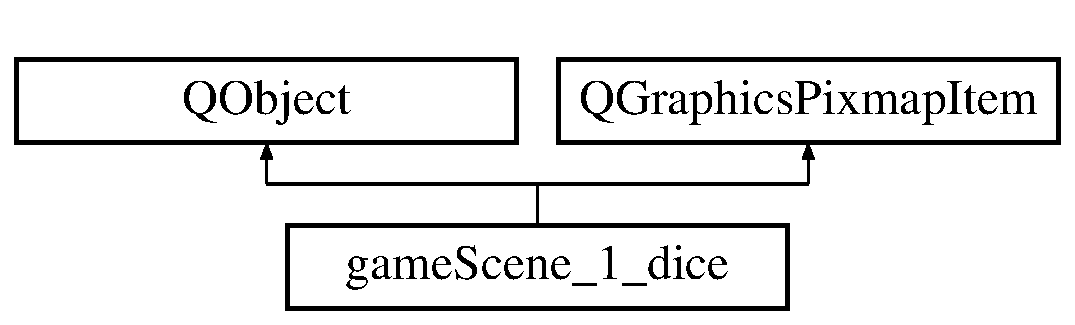
\includegraphics[height=2.000000cm]{classgameScene__1__dice}
\end{center}
\end{figure}
\subsection*{Public Slots}
\begin{DoxyCompactItemize}
\item 
void \hyperlink{classgameScene__1__dice_aa70064b1cab5ac14ca1a7ff757a1e73b}{update} ()
\begin{DoxyCompactList}\small\item\em \hyperlink{classgameScene__1__dice_aa70064b1cab5ac14ca1a7ff757a1e73b}{game\-Scene\-\_\-1\-\_\-dice\-::update} \end{DoxyCompactList}\item 
void \hyperlink{classgameScene__1__dice_af16a75f80f77a5ef743eb0e458ad40fd}{setup} (int value)
\begin{DoxyCompactList}\small\item\em \hyperlink{classgameScene__1__dice_af16a75f80f77a5ef743eb0e458ad40fd}{game\-Scene\-\_\-1\-\_\-dice\-::setup} \end{DoxyCompactList}\end{DoxyCompactItemize}
\subsection*{Public Member Functions}
\begin{DoxyCompactItemize}
\item 
\hypertarget{classgameScene__1__dice_a0344f480bb7de748b55dabe760db0e80}{{\bfseries game\-Scene\-\_\-1\-\_\-dice} (Q\-Object $\ast$parent=0)}\label{classgameScene__1__dice_a0344f480bb7de748b55dabe760db0e80}

\end{DoxyCompactItemize}
\subsection*{Public Attributes}
\begin{DoxyCompactItemize}
\item 
\hypertarget{classgameScene__1__dice_a3b5c0dd706e762b7655b302b2617a5bb}{int $\ast$ \hyperlink{classgameScene__1__dice_a3b5c0dd706e762b7655b302b2617a5bb}{id}}\label{classgameScene__1__dice_a3b5c0dd706e762b7655b302b2617a5bb}

\begin{DoxyCompactList}\small\item\em I\-D of the dice ( dice1/dice2) \end{DoxyCompactList}\item 
\hypertarget{classgameScene__1__dice_a5519f90954e1a845e28f316a71fe3cf6}{int $\ast$ \hyperlink{classgameScene__1__dice_a5519f90954e1a845e28f316a71fe3cf6}{dice\-Val}}\label{classgameScene__1__dice_a5519f90954e1a845e28f316a71fe3cf6}

\begin{DoxyCompactList}\small\item\em int denoting current value of dice \end{DoxyCompactList}\end{DoxyCompactItemize}


\subsection{Member Function Documentation}
\hypertarget{classgameScene__1__dice_af16a75f80f77a5ef743eb0e458ad40fd}{\index{game\-Scene\-\_\-1\-\_\-dice@{game\-Scene\-\_\-1\-\_\-dice}!setup@{setup}}
\index{setup@{setup}!gameScene_1_dice@{game\-Scene\-\_\-1\-\_\-dice}}
\subsubsection[{setup}]{\setlength{\rightskip}{0pt plus 5cm}void game\-Scene\-\_\-1\-\_\-dice\-::setup (
\begin{DoxyParamCaption}
\item[{int}]{value}
\end{DoxyParamCaption}
)\hspace{0.3cm}{\ttfamily [slot]}}}\label{classgameScene__1__dice_af16a75f80f77a5ef743eb0e458ad40fd}


\hyperlink{classgameScene__1__dice_af16a75f80f77a5ef743eb0e458ad40fd}{game\-Scene\-\_\-1\-\_\-dice\-::setup} 


\begin{DoxyParams}{Parameters}
{\em value} & \-: id of dice (either 1 or 2)\\
\hline
\end{DoxyParams}
Setup a dice instance \hypertarget{classgameScene__1__dice_aa70064b1cab5ac14ca1a7ff757a1e73b}{\index{game\-Scene\-\_\-1\-\_\-dice@{game\-Scene\-\_\-1\-\_\-dice}!update@{update}}
\index{update@{update}!gameScene_1_dice@{game\-Scene\-\_\-1\-\_\-dice}}
\subsubsection[{update}]{\setlength{\rightskip}{0pt plus 5cm}void game\-Scene\-\_\-1\-\_\-dice\-::update (
\begin{DoxyParamCaption}
{}
\end{DoxyParamCaption}
)\hspace{0.3cm}{\ttfamily [slot]}}}\label{classgameScene__1__dice_aa70064b1cab5ac14ca1a7ff757a1e73b}


\hyperlink{classgameScene__1__dice_aa70064b1cab5ac14ca1a7ff757a1e73b}{game\-Scene\-\_\-1\-\_\-dice\-::update} 

Roll the dice and update its value randomly 

The documentation for this class was generated from the following files\-:\begin{DoxyCompactItemize}
\item 
\hyperlink{gamescene__1__dice_8h}{gamescene\-\_\-1\-\_\-dice.\-h}\item 
gamescene\-\_\-1\-\_\-dice.\-cpp\end{DoxyCompactItemize}

\hypertarget{classgamescene__1__ladderSnake}{\section{gamescene\-\_\-1\-\_\-ladder\-Snake Class Reference}
\label{classgamescene__1__ladderSnake}\index{gamescene\-\_\-1\-\_\-ladder\-Snake@{gamescene\-\_\-1\-\_\-ladder\-Snake}}
}
Inheritance diagram for gamescene\-\_\-1\-\_\-ladder\-Snake\-:\begin{figure}[H]
\begin{center}
\leavevmode
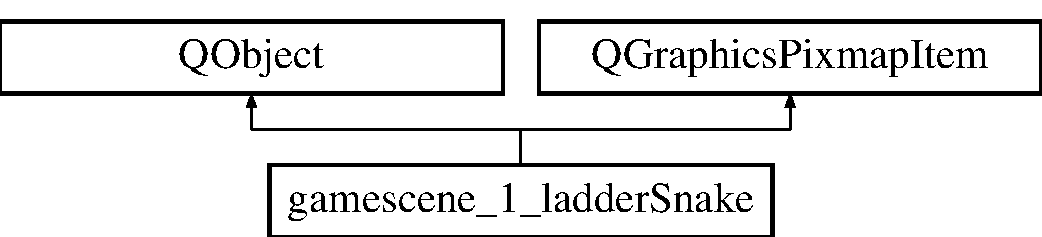
\includegraphics[height=2.000000cm]{classgamescene__1__ladderSnake}
\end{center}
\end{figure}
\subsection*{Public Slots}
\begin{DoxyCompactItemize}
\item 
void \hyperlink{classgamescene__1__ladderSnake_a035cdb1009cf47abbe272ebcffb9ae3a}{init\-Ladder} (int seed, int start, int end)
\begin{DoxyCompactList}\small\item\em \hyperlink{classgamescene__1__ladderSnake_a035cdb1009cf47abbe272ebcffb9ae3a}{gamescene\-\_\-1\-\_\-ladder\-Snake\-::init\-Ladder} \end{DoxyCompactList}\item 
int \hyperlink{classgamescene__1__ladderSnake_a80c04a3bc2387a0760ac5dcc52fc3086}{get\-X\-Ycase} (int case\-Num, int xy)
\begin{DoxyCompactList}\small\item\em \hyperlink{classgamescene__1__ladderSnake_a80c04a3bc2387a0760ac5dcc52fc3086}{gamescene\-\_\-1\-\_\-ladder\-Snake\-::get\-X\-Ycase} \end{DoxyCompactList}\end{DoxyCompactItemize}
\subsection*{Public Member Functions}
\begin{DoxyCompactItemize}
\item 
\hypertarget{classgamescene__1__ladderSnake_ae38ad9fce246708c2229806145421ed3}{{\bfseries gamescene\-\_\-1\-\_\-ladder\-Snake} (Q\-Object $\ast$parent=0)}\label{classgamescene__1__ladderSnake_ae38ad9fce246708c2229806145421ed3}

\end{DoxyCompactItemize}
\subsection*{Public Attributes}
\begin{DoxyCompactItemize}
\item 
\hypertarget{classgamescene__1__ladderSnake_a9f6d4f80e42294baf24e9f75595f2f36}{Q\-Pixmap $\ast$ \hyperlink{classgamescene__1__ladderSnake_a9f6d4f80e42294baf24e9f75595f2f36}{image}}\label{classgamescene__1__ladderSnake_a9f6d4f80e42294baf24e9f75595f2f36}

\begin{DoxyCompactList}\small\item\em Image associated to ladder/snake. \end{DoxyCompactList}\item 
\hypertarget{classgamescene__1__ladderSnake_a84c434594befd54905917da864b842f5}{int $\ast$ \hyperlink{classgamescene__1__ladderSnake_a84c434594befd54905917da864b842f5}{id}}\label{classgamescene__1__ladderSnake_a84c434594befd54905917da864b842f5}

\begin{DoxyCompactList}\small\item\em Id associated to ladder/snake. \end{DoxyCompactList}\item 
\hypertarget{classgamescene__1__ladderSnake_a4412cbb937c7acdb62f70fb1c348b315}{bool $\ast$ \hyperlink{classgamescene__1__ladderSnake_a4412cbb937c7acdb62f70fb1c348b315}{go\-Forward}}\label{classgamescene__1__ladderSnake_a4412cbb937c7acdb62f70fb1c348b315}

\begin{DoxyCompactList}\small\item\em Bool associated to movement logic. \end{DoxyCompactList}\item 
\hypertarget{classgamescene__1__ladderSnake_ad521dbf1e24a90ccb3e1d9ffca2cd110}{int $\ast$ \hyperlink{classgamescene__1__ladderSnake_ad521dbf1e24a90ccb3e1d9ffca2cd110}{pos\-Xstart}}\label{classgamescene__1__ladderSnake_ad521dbf1e24a90ccb3e1d9ffca2cd110}

\begin{DoxyCompactList}\small\item\em Temp value used in calculations across functions. \end{DoxyCompactList}\item 
\hypertarget{classgamescene__1__ladderSnake_a96d4e6756e756f79cb4eebfa24a4f6fb}{int $\ast$ \hyperlink{classgamescene__1__ladderSnake_a96d4e6756e756f79cb4eebfa24a4f6fb}{pos\-Xend}}\label{classgamescene__1__ladderSnake_a96d4e6756e756f79cb4eebfa24a4f6fb}

\begin{DoxyCompactList}\small\item\em Temp value used in calculations across functions. \end{DoxyCompactList}\item 
\hypertarget{classgamescene__1__ladderSnake_afbfb7c101342e8875a5f92aae5d0145d}{int $\ast$ \hyperlink{classgamescene__1__ladderSnake_afbfb7c101342e8875a5f92aae5d0145d}{pos\-Ystart}}\label{classgamescene__1__ladderSnake_afbfb7c101342e8875a5f92aae5d0145d}

\begin{DoxyCompactList}\small\item\em Temp value used in calculations across functions. \end{DoxyCompactList}\item 
\hypertarget{classgamescene__1__ladderSnake_a0305757722dba83cbbc72b7d616b8453}{int $\ast$ \hyperlink{classgamescene__1__ladderSnake_a0305757722dba83cbbc72b7d616b8453}{pos\-Yend}}\label{classgamescene__1__ladderSnake_a0305757722dba83cbbc72b7d616b8453}

\begin{DoxyCompactList}\small\item\em Temp value used in calculations across functions. \end{DoxyCompactList}\item 
\hypertarget{classgamescene__1__ladderSnake_a5ca42a82f5abaece614f71eb6cf51551}{int $\ast$ \hyperlink{classgamescene__1__ladderSnake_a5ca42a82f5abaece614f71eb6cf51551}{pos\-Xtemp}}\label{classgamescene__1__ladderSnake_a5ca42a82f5abaece614f71eb6cf51551}

\begin{DoxyCompactList}\small\item\em Temp value used in calculations across functions. \end{DoxyCompactList}\item 
\hypertarget{classgamescene__1__ladderSnake_a6dfe0e78a12b63efc2178fcbedfbe2d4}{int $\ast$ \hyperlink{classgamescene__1__ladderSnake_a6dfe0e78a12b63efc2178fcbedfbe2d4}{pos\-Ytemp}}\label{classgamescene__1__ladderSnake_a6dfe0e78a12b63efc2178fcbedfbe2d4}

\begin{DoxyCompactList}\small\item\em Temp value used in calculations across functions. \end{DoxyCompactList}\item 
\hypertarget{classgamescene__1__ladderSnake_a712b23de16d8d538a054184467007904}{int $\ast$ \hyperlink{classgamescene__1__ladderSnake_a712b23de16d8d538a054184467007904}{pos\-Xtemp\-Func}}\label{classgamescene__1__ladderSnake_a712b23de16d8d538a054184467007904}

\begin{DoxyCompactList}\small\item\em Temp value used in calculations across functions. \end{DoxyCompactList}\item 
\hypertarget{classgamescene__1__ladderSnake_ac490aecde4bcea372216a7aa09fac13f}{int $\ast$ \hyperlink{classgamescene__1__ladderSnake_ac490aecde4bcea372216a7aa09fac13f}{pos\-Ytemp\-Func}}\label{classgamescene__1__ladderSnake_ac490aecde4bcea372216a7aa09fac13f}

\begin{DoxyCompactList}\small\item\em Temp value used in calculations across functions. \end{DoxyCompactList}\item 
\hypertarget{classgamescene__1__ladderSnake_acd9d50c3aa4c03f9db9ae1cee3b3283d}{double $\ast$ \hyperlink{classgamescene__1__ladderSnake_acd9d50c3aa4c03f9db9ae1cee3b3283d}{size}}\label{classgamescene__1__ladderSnake_acd9d50c3aa4c03f9db9ae1cee3b3283d}

\begin{DoxyCompactList}\small\item\em Temp value used in calculations across functions. \end{DoxyCompactList}\item 
\hypertarget{classgamescene__1__ladderSnake_acef81d50d4cd4e0168c26b5b0347c964}{double $\ast$ \hyperlink{classgamescene__1__ladderSnake_acef81d50d4cd4e0168c26b5b0347c964}{angle}}\label{classgamescene__1__ladderSnake_acef81d50d4cd4e0168c26b5b0347c964}

\begin{DoxyCompactList}\small\item\em Temp value used in calculations across functions. \end{DoxyCompactList}\item 
\hypertarget{classgamescene__1__ladderSnake_a8f56ae5b63fa153006ba2f0233a73b9d}{double $\ast$ \hyperlink{classgamescene__1__ladderSnake_a8f56ae5b63fa153006ba2f0233a73b9d}{center\-X}}\label{classgamescene__1__ladderSnake_a8f56ae5b63fa153006ba2f0233a73b9d}

\begin{DoxyCompactList}\small\item\em Temp value used in calculations across functions. \end{DoxyCompactList}\item 
\hypertarget{classgamescene__1__ladderSnake_a74d54191e673db2dde4396c2a50c6989}{double $\ast$ \hyperlink{classgamescene__1__ladderSnake_a74d54191e673db2dde4396c2a50c6989}{center\-Y}}\label{classgamescene__1__ladderSnake_a74d54191e673db2dde4396c2a50c6989}

\begin{DoxyCompactList}\small\item\em Temp value used in calculations across functions. \end{DoxyCompactList}\item 
\hypertarget{classgamescene__1__ladderSnake_a998eb0a715d26b013f3f7ecc698d537f}{double $\ast$ \hyperlink{classgamescene__1__ladderSnake_a998eb0a715d26b013f3f7ecc698d537f}{temp\-Length}}\label{classgamescene__1__ladderSnake_a998eb0a715d26b013f3f7ecc698d537f}

\begin{DoxyCompactList}\small\item\em Temp value used in calculations across functions. \end{DoxyCompactList}\end{DoxyCompactItemize}


\subsection{Member Function Documentation}
\hypertarget{classgamescene__1__ladderSnake_a80c04a3bc2387a0760ac5dcc52fc3086}{\index{gamescene\-\_\-1\-\_\-ladder\-Snake@{gamescene\-\_\-1\-\_\-ladder\-Snake}!get\-X\-Ycase@{get\-X\-Ycase}}
\index{get\-X\-Ycase@{get\-X\-Ycase}!gamescene_1_ladderSnake@{gamescene\-\_\-1\-\_\-ladder\-Snake}}
\subsubsection[{get\-X\-Ycase}]{\setlength{\rightskip}{0pt plus 5cm}int gamescene\-\_\-1\-\_\-ladder\-Snake\-::get\-X\-Ycase (
\begin{DoxyParamCaption}
\item[{int}]{case\-Num, }
\item[{int}]{xy}
\end{DoxyParamCaption}
)\hspace{0.3cm}{\ttfamily [slot]}}}\label{classgamescene__1__ladderSnake_a80c04a3bc2387a0760ac5dcc52fc3086}


\hyperlink{classgamescene__1__ladderSnake_a80c04a3bc2387a0760ac5dcc52fc3086}{gamescene\-\_\-1\-\_\-ladder\-Snake\-::get\-X\-Ycase} 


\begin{DoxyParams}{Parameters}
{\em case\-Num} & \-: value of the case to search \\
\hline
{\em xy} & \-: xy=0 return x value , xy=1 return y value \\
\hline
\end{DoxyParams}
\begin{DoxyReturn}{Returns}
x coordinate of the case
\end{DoxyReturn}
When assigning a case to a ladder/snake, we search for its coordinates using this function \hypertarget{classgamescene__1__ladderSnake_a035cdb1009cf47abbe272ebcffb9ae3a}{\index{gamescene\-\_\-1\-\_\-ladder\-Snake@{gamescene\-\_\-1\-\_\-ladder\-Snake}!init\-Ladder@{init\-Ladder}}
\index{init\-Ladder@{init\-Ladder}!gamescene_1_ladderSnake@{gamescene\-\_\-1\-\_\-ladder\-Snake}}
\subsubsection[{init\-Ladder}]{\setlength{\rightskip}{0pt plus 5cm}void gamescene\-\_\-1\-\_\-ladder\-Snake\-::init\-Ladder (
\begin{DoxyParamCaption}
\item[{int}]{seed, }
\item[{int}]{start, }
\item[{int}]{end}
\end{DoxyParamCaption}
)\hspace{0.3cm}{\ttfamily [slot]}}}\label{classgamescene__1__ladderSnake_a035cdb1009cf47abbe272ebcffb9ae3a}


\hyperlink{classgamescene__1__ladderSnake_a035cdb1009cf47abbe272ebcffb9ae3a}{gamescene\-\_\-1\-\_\-ladder\-Snake\-::init\-Ladder} 


\begin{DoxyParams}{Parameters}
{\em seed} & \-: 0-\/1 are ladder instance seeds, 2-\/3-\/4 are snake instance seeds \\
\hline
{\em start} & \-: where is the instance start position \\
\hline
{\em end} & \-: where is the instance end position\\
\hline
\end{DoxyParams}
Initialize ladder or snake instance with given parameters 

The documentation for this class was generated from the following files\-:\begin{DoxyCompactItemize}
\item 
gamescene\-\_\-1\-\_\-ladder\-Snake.\-h\item 
gamescene\-\_\-1\-\_\-ladder\-Snake.\-cpp\end{DoxyCompactItemize}

\hypertarget{classgameScene__1__player}{\section{game\-Scene\-\_\-1\-\_\-player Class Reference}
\label{classgameScene__1__player}\index{game\-Scene\-\_\-1\-\_\-player@{game\-Scene\-\_\-1\-\_\-player}}
}
Inheritance diagram for game\-Scene\-\_\-1\-\_\-player\-:\begin{figure}[H]
\begin{center}
\leavevmode
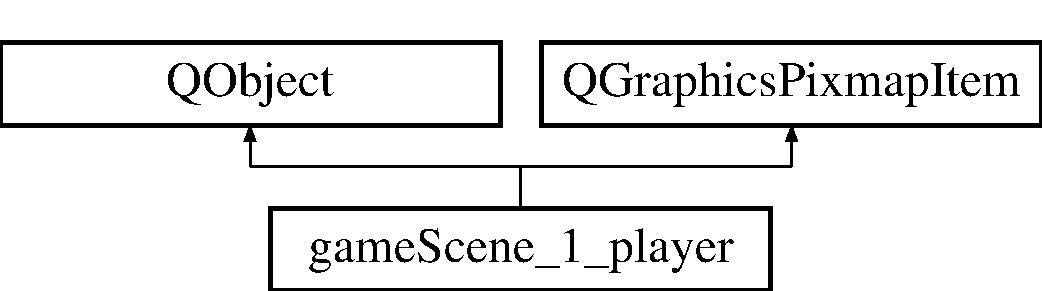
\includegraphics[height=2.000000cm]{classgameScene__1__player}
\end{center}
\end{figure}
\subsection*{Public Slots}
\begin{DoxyCompactItemize}
\item 
void \hyperlink{classgameScene__1__player_a3853a587d2dab9fcaa90f2c614e27b16}{move\-Instantaneous} ()
\begin{DoxyCompactList}\small\item\em \hyperlink{classgameScene__1__player_a3853a587d2dab9fcaa90f2c614e27b16}{game\-Scene\-\_\-1\-\_\-player\-::move\-Instantaneous} \end{DoxyCompactList}\item 
void \hyperlink{classgameScene__1__player_a00915de85128384e57721fb4b4f1b84c}{setup} (int playerid)
\begin{DoxyCompactList}\small\item\em \hyperlink{classgameScene__1__player_a00915de85128384e57721fb4b4f1b84c}{game\-Scene\-\_\-1\-\_\-player\-::setup} \end{DoxyCompactList}\end{DoxyCompactItemize}
\subsection*{Public Member Functions}
\begin{DoxyCompactItemize}
\item 
\hypertarget{classgameScene__1__player_a406e5938fd1904873a812106b8a68eb7}{{\bfseries game\-Scene\-\_\-1\-\_\-player} (Q\-Object $\ast$parent=0)}\label{classgameScene__1__player_a406e5938fd1904873a812106b8a68eb7}

\end{DoxyCompactItemize}
\subsection*{Public Attributes}
\begin{DoxyCompactItemize}
\item 
\hypertarget{classgameScene__1__player_a703e0820652547f52908ce7d4df714bc}{Q\-Graphics\-Scene $\ast$ {\bfseries parent\-Scene}}\label{classgameScene__1__player_a703e0820652547f52908ce7d4df714bc}

\item 
\hypertarget{classgameScene__1__player_a3be5c24385d356351b9d315ebf47ebe2}{bool $\ast$ \hyperlink{classgameScene__1__player_a3be5c24385d356351b9d315ebf47ebe2}{go\-Forward}}\label{classgameScene__1__player_a3be5c24385d356351b9d315ebf47ebe2}

\begin{DoxyCompactList}\small\item\em Bool used in movement logic. \end{DoxyCompactList}\item 
\hypertarget{classgameScene__1__player_a4e8692a39c422daee4b8c8d7179e9d0c}{int $\ast$ \hyperlink{classgameScene__1__player_a4e8692a39c422daee4b8c8d7179e9d0c}{id}}\label{classgameScene__1__player_a4e8692a39c422daee4b8c8d7179e9d0c}

\begin{DoxyCompactList}\small\item\em I\-D used for player1/player2. \end{DoxyCompactList}\item 
\hypertarget{classgameScene__1__player_a1ef73975a59adf58a5777fb2629ec6b9}{int $\ast$ \hyperlink{classgameScene__1__player_a1ef73975a59adf58a5777fb2629ec6b9}{position}}\label{classgameScene__1__player_a1ef73975a59adf58a5777fb2629ec6b9}

\begin{DoxyCompactList}\small\item\em Used to store player position. \end{DoxyCompactList}\item 
\hypertarget{classgameScene__1__player_a232a310c7b60dc3c4c082d1e7be35b27}{int $\ast$ \hyperlink{classgameScene__1__player_a232a310c7b60dc3c4c082d1e7be35b27}{new\-Position}}\label{classgameScene__1__player_a232a310c7b60dc3c4c082d1e7be35b27}

\begin{DoxyCompactList}\small\item\em Used to store player position. \end{DoxyCompactList}\end{DoxyCompactItemize}


\subsection{Member Function Documentation}
\hypertarget{classgameScene__1__player_a3853a587d2dab9fcaa90f2c614e27b16}{\index{game\-Scene\-\_\-1\-\_\-player@{game\-Scene\-\_\-1\-\_\-player}!move\-Instantaneous@{move\-Instantaneous}}
\index{move\-Instantaneous@{move\-Instantaneous}!gameScene_1_player@{game\-Scene\-\_\-1\-\_\-player}}
\subsubsection[{move\-Instantaneous}]{\setlength{\rightskip}{0pt plus 5cm}void game\-Scene\-\_\-1\-\_\-player\-::move\-Instantaneous (
\begin{DoxyParamCaption}
{}
\end{DoxyParamCaption}
)\hspace{0.3cm}{\ttfamily [slot]}}}\label{classgameScene__1__player_a3853a587d2dab9fcaa90f2c614e27b16}


\hyperlink{classgameScene__1__player_a3853a587d2dab9fcaa90f2c614e27b16}{game\-Scene\-\_\-1\-\_\-player\-::move\-Instantaneous} 

Move the player to its newly assigned position \hypertarget{classgameScene__1__player_a00915de85128384e57721fb4b4f1b84c}{\index{game\-Scene\-\_\-1\-\_\-player@{game\-Scene\-\_\-1\-\_\-player}!setup@{setup}}
\index{setup@{setup}!gameScene_1_player@{game\-Scene\-\_\-1\-\_\-player}}
\subsubsection[{setup}]{\setlength{\rightskip}{0pt plus 5cm}void game\-Scene\-\_\-1\-\_\-player\-::setup (
\begin{DoxyParamCaption}
\item[{int}]{playerid}
\end{DoxyParamCaption}
)\hspace{0.3cm}{\ttfamily [slot]}}}\label{classgameScene__1__player_a00915de85128384e57721fb4b4f1b84c}


\hyperlink{classgameScene__1__player_a00915de85128384e57721fb4b4f1b84c}{game\-Scene\-\_\-1\-\_\-player\-::setup} 


\begin{DoxyParams}{Parameters}
{\em playerid} & \-: id for player\\
\hline
\end{DoxyParams}
Initializing the player instance 

The documentation for this class was generated from the following files\-:\begin{DoxyCompactItemize}
\item 
gamescene\-\_\-1\-\_\-player.\-h\item 
gamescene\-\_\-1\-\_\-player.\-cpp\end{DoxyCompactItemize}

\hypertarget{classloginWidget}{\section{login\-Widget Class Reference}
\label{classloginWidget}\index{login\-Widget@{login\-Widget}}
}
Inheritance diagram for login\-Widget\-:\begin{figure}[H]
\begin{center}
\leavevmode
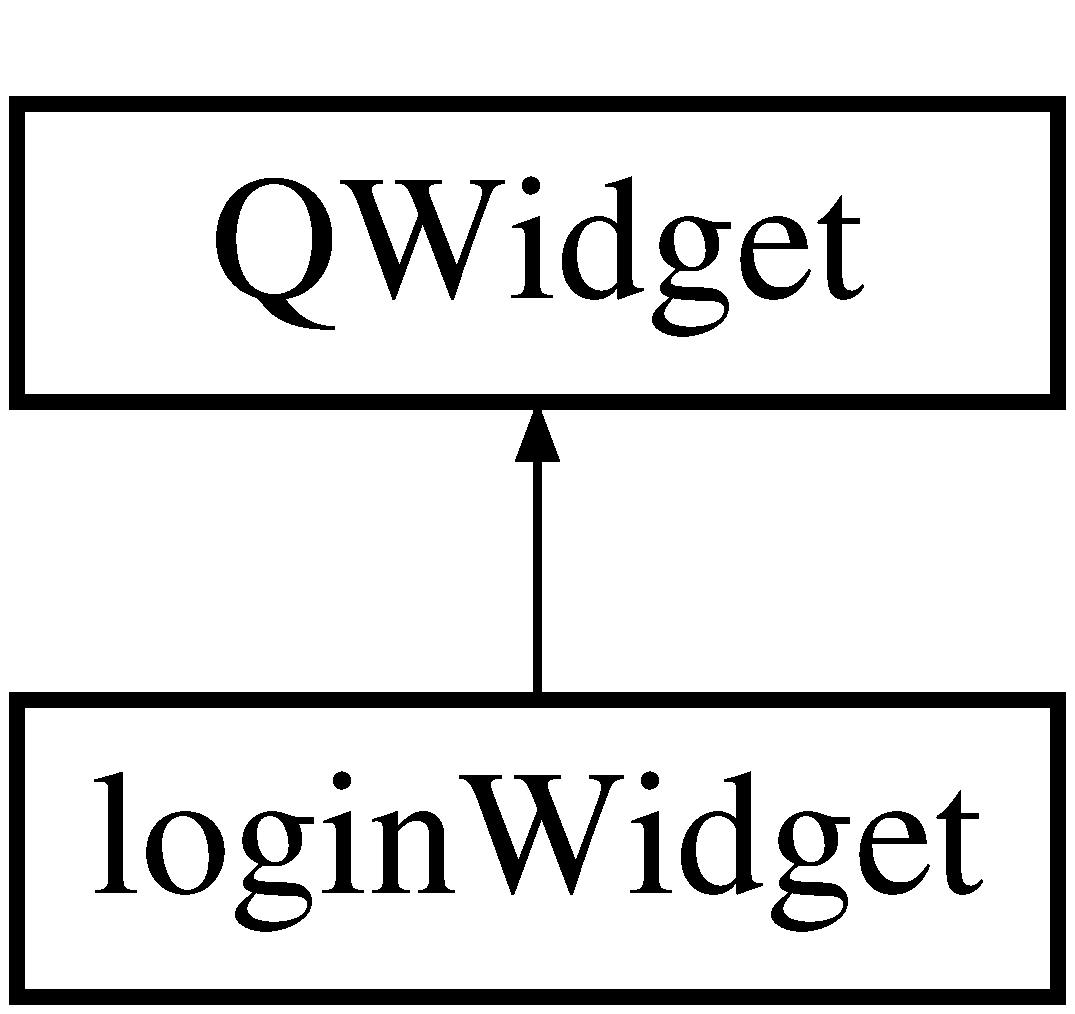
\includegraphics[height=2.000000cm]{classloginWidget}
\end{center}
\end{figure}
\subsection*{Public Slots}
\begin{DoxyCompactItemize}
\item 
void \hyperlink{classloginWidget_afcb096399c33f93111861cf221c833bb}{Go\-To\-Register\-Page} ()
\begin{DoxyCompactList}\small\item\em \hyperlink{classloginWidget_afcb096399c33f93111861cf221c833bb}{login\-Widget\-::\-Go\-To\-Register\-Page} \end{DoxyCompactList}\item 
void \hyperlink{classloginWidget_afbc51bef452e79a14eeaf3fbd3c716ec}{check\-Login} ()
\begin{DoxyCompactList}\small\item\em \hyperlink{classloginWidget_afbc51bef452e79a14eeaf3fbd3c716ec}{login\-Widget\-::check\-Login} \end{DoxyCompactList}\item 
void \hyperlink{classloginWidget_ab19c0e07c66cdbf37ebd73d32c4c581d}{Go\-To\-Main\-As\-Guest} ()
\begin{DoxyCompactList}\small\item\em \hyperlink{classloginWidget_ab19c0e07c66cdbf37ebd73d32c4c581d}{login\-Widget\-::\-Go\-To\-Main\-As\-Guest} \end{DoxyCompactList}\end{DoxyCompactItemize}
\subsection*{Public Member Functions}
\begin{DoxyCompactItemize}
\item 
\hypertarget{classloginWidget_a4fc020d7888ff7ed679629e39c362732}{{\bfseries login\-Widget} (Q\-Widget $\ast$parent=0)}\label{classloginWidget_a4fc020d7888ff7ed679629e39c362732}

\end{DoxyCompactItemize}
\subsection*{Public Attributes}
\begin{DoxyCompactItemize}
\item 
\hypertarget{classloginWidget_adfa3f06d5859e8f9b6485aeaa494a8f6}{Q\-Label $\ast$ \hyperlink{classloginWidget_adfa3f06d5859e8f9b6485aeaa494a8f6}{test\-\_\-screen}}\label{classloginWidget_adfa3f06d5859e8f9b6485aeaa494a8f6}

\begin{DoxyCompactList}\small\item\em Text label. \end{DoxyCompactList}\item 
\hypertarget{classloginWidget_a838df9541b3962474f735893dfc91514}{Q\-Push\-Button $\ast$ \hyperlink{classloginWidget_a838df9541b3962474f735893dfc91514}{Log\-I\-Nbutton}}\label{classloginWidget_a838df9541b3962474f735893dfc91514}

\begin{DoxyCompactList}\small\item\em Menu button to login. \end{DoxyCompactList}\item 
\hypertarget{classloginWidget_aaf5abfa2347947c911400274d83a9b59}{Q\-Push\-Button $\ast$ \hyperlink{classloginWidget_aaf5abfa2347947c911400274d83a9b59}{Register\-Button}}\label{classloginWidget_aaf5abfa2347947c911400274d83a9b59}

\begin{DoxyCompactList}\small\item\em Menu button to register. \end{DoxyCompactList}\item 
\hypertarget{classloginWidget_a81bd16c8e012bb293d3c884760c88fb1}{Q\-Grid\-Layout $\ast$ \hyperlink{classloginWidget_a81bd16c8e012bb293d3c884760c88fb1}{test\-\_\-layout}}\label{classloginWidget_a81bd16c8e012bb293d3c884760c88fb1}

\begin{DoxyCompactList}\small\item\em Main Layout. \end{DoxyCompactList}\item 
\hypertarget{classloginWidget_ad253acb27c0ba1bfc00416b100ccbcbf}{Q\-Label $\ast$ \hyperlink{classloginWidget_ad253acb27c0ba1bfc00416b100ccbcbf}{User\-Name}}\label{classloginWidget_ad253acb27c0ba1bfc00416b100ccbcbf}

\begin{DoxyCompactList}\small\item\em Text label. \end{DoxyCompactList}\item 
\hypertarget{classloginWidget_a091bc8135793361cd5212d770d47d9f6}{Q\-Label $\ast$ \hyperlink{classloginWidget_a091bc8135793361cd5212d770d47d9f6}{Pass\-Word}}\label{classloginWidget_a091bc8135793361cd5212d770d47d9f6}

\begin{DoxyCompactList}\small\item\em Text label. \end{DoxyCompactList}\item 
\hypertarget{classloginWidget_a0063152147c8ffb1def2ee9dc83bfb13}{Q\-Line\-Edit $\ast$ \hyperlink{classloginWidget_a0063152147c8ffb1def2ee9dc83bfb13}{User\-Name\-Line}}\label{classloginWidget_a0063152147c8ffb1def2ee9dc83bfb13}

\begin{DoxyCompactList}\small\item\em Line edit field. \end{DoxyCompactList}\item 
\hypertarget{classloginWidget_a8b2562b3a80b846814e68e4e646fe597}{Q\-Line\-Edit $\ast$ \hyperlink{classloginWidget_a8b2562b3a80b846814e68e4e646fe597}{Pass\-Word\-Line}}\label{classloginWidget_a8b2562b3a80b846814e68e4e646fe597}

\begin{DoxyCompactList}\small\item\em Line edit field. \end{DoxyCompactList}\item 
\hypertarget{classloginWidget_a0a16f61332cb4b47c0869a98fa180fd8}{Q\-Label $\ast$ \hyperlink{classloginWidget_a0a16f61332cb4b47c0869a98fa180fd8}{Error\-Message}}\label{classloginWidget_a0a16f61332cb4b47c0869a98fa180fd8}

\begin{DoxyCompactList}\small\item\em Text label. \end{DoxyCompactList}\item 
\hypertarget{classloginWidget_ad6d4c65a10444007bfb47c7bd87e61cd}{Q\-Push\-Button $\ast$ \hyperlink{classloginWidget_ad6d4c65a10444007bfb47c7bd87e61cd}{Play\-As\-Guest\-Button}}\label{classloginWidget_ad6d4c65a10444007bfb47c7bd87e61cd}

\begin{DoxyCompactList}\small\item\em Menu button to play as guest. \end{DoxyCompactList}\end{DoxyCompactItemize}


\subsection{Member Function Documentation}
\hypertarget{classloginWidget_afbc51bef452e79a14eeaf3fbd3c716ec}{\index{login\-Widget@{login\-Widget}!check\-Login@{check\-Login}}
\index{check\-Login@{check\-Login}!loginWidget@{login\-Widget}}
\subsubsection[{check\-Login}]{\setlength{\rightskip}{0pt plus 5cm}void login\-Widget\-::check\-Login (
\begin{DoxyParamCaption}
{}
\end{DoxyParamCaption}
)\hspace{0.3cm}{\ttfamily [slot]}}}\label{classloginWidget_afbc51bef452e79a14eeaf3fbd3c716ec}


\hyperlink{classloginWidget_afbc51bef452e79a14eeaf3fbd3c716ec}{login\-Widget\-::check\-Login} 

Check if login conditions are met, and login with a particular user \hypertarget{classloginWidget_ab19c0e07c66cdbf37ebd73d32c4c581d}{\index{login\-Widget@{login\-Widget}!Go\-To\-Main\-As\-Guest@{Go\-To\-Main\-As\-Guest}}
\index{Go\-To\-Main\-As\-Guest@{Go\-To\-Main\-As\-Guest}!loginWidget@{login\-Widget}}
\subsubsection[{Go\-To\-Main\-As\-Guest}]{\setlength{\rightskip}{0pt plus 5cm}void login\-Widget\-::\-Go\-To\-Main\-As\-Guest (
\begin{DoxyParamCaption}
{}
\end{DoxyParamCaption}
)\hspace{0.3cm}{\ttfamily [slot]}}}\label{classloginWidget_ab19c0e07c66cdbf37ebd73d32c4c581d}


\hyperlink{classloginWidget_ab19c0e07c66cdbf37ebd73d32c4c581d}{login\-Widget\-::\-Go\-To\-Main\-As\-Guest} 

Open main menu as a guest \hypertarget{classloginWidget_afcb096399c33f93111861cf221c833bb}{\index{login\-Widget@{login\-Widget}!Go\-To\-Register\-Page@{Go\-To\-Register\-Page}}
\index{Go\-To\-Register\-Page@{Go\-To\-Register\-Page}!loginWidget@{login\-Widget}}
\subsubsection[{Go\-To\-Register\-Page}]{\setlength{\rightskip}{0pt plus 5cm}void login\-Widget\-::\-Go\-To\-Register\-Page (
\begin{DoxyParamCaption}
{}
\end{DoxyParamCaption}
)\hspace{0.3cm}{\ttfamily [slot]}}}\label{classloginWidget_afcb096399c33f93111861cf221c833bb}


\hyperlink{classloginWidget_afcb096399c33f93111861cf221c833bb}{login\-Widget\-::\-Go\-To\-Register\-Page} 

Load up register page 

The documentation for this class was generated from the following files\-:\begin{DoxyCompactItemize}
\item 
loginwidget.\-h\item 
loginwidget.\-cpp\end{DoxyCompactItemize}

\hypertarget{classmenuWidget}{\section{menu\-Widget Class Reference}
\label{classmenuWidget}\index{menu\-Widget@{menu\-Widget}}
}
Inheritance diagram for menu\-Widget\-:\begin{figure}[H]
\begin{center}
\leavevmode
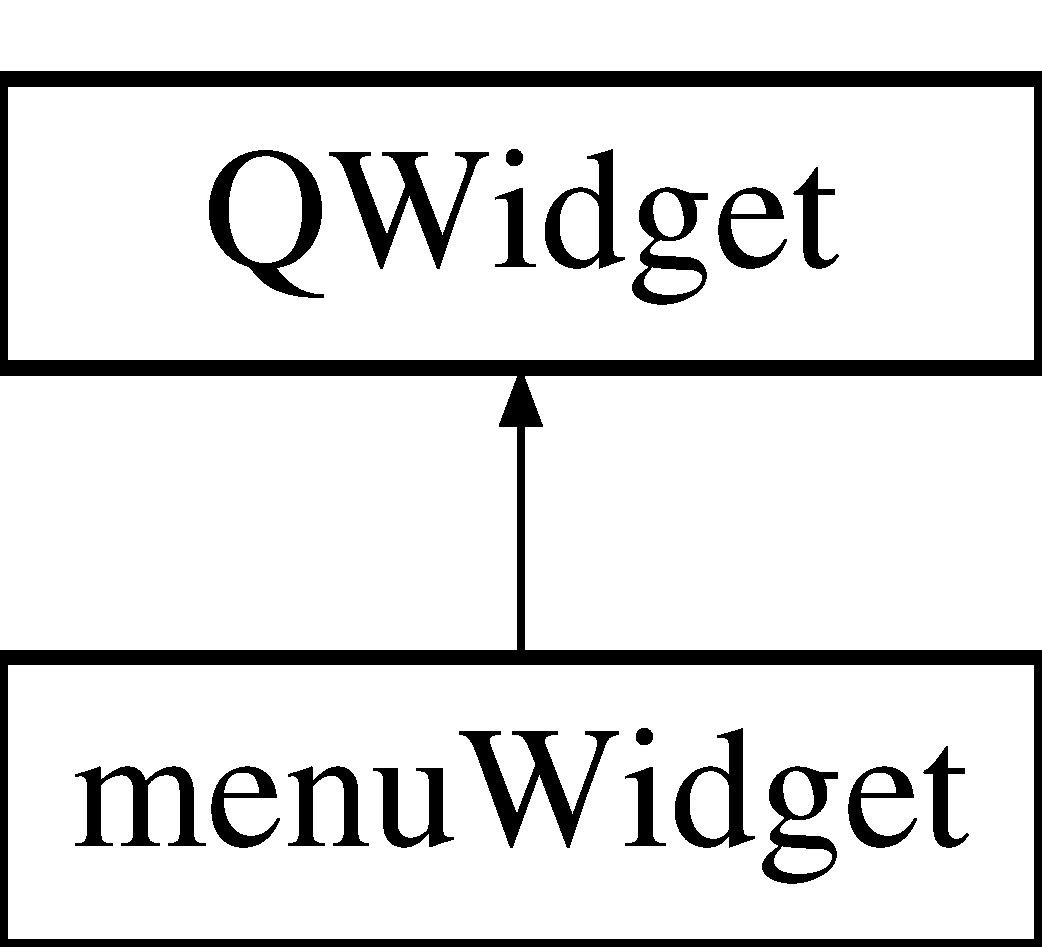
\includegraphics[height=2.000000cm]{classmenuWidget}
\end{center}
\end{figure}
\subsection*{Public Slots}
\begin{DoxyCompactItemize}
\item 
void \hyperlink{classmenuWidget_a3380372012023661288a213ba4b4a863}{read\-From\-Json\-Profile} ()
\begin{DoxyCompactList}\small\item\em \hyperlink{classmenuWidget_a3380372012023661288a213ba4b4a863}{menu\-Widget\-::read\-From\-Json\-Profile} \end{DoxyCompactList}\item 
\hypertarget{classmenuWidget_a0f1b8132d994d08682389e2a344a36ba}{void {\bfseries logout} ()}\label{classmenuWidget_a0f1b8132d994d08682389e2a344a36ba}

\item 
void \hyperlink{classmenuWidget_ad5ec96474e3d43c8e011b5c38a596b23}{start\-Game\-C\-P\-U} ()
\begin{DoxyCompactList}\small\item\em \hyperlink{classmenuWidget_ad5ec96474e3d43c8e011b5c38a596b23}{menu\-Widget\-::start\-Game\-C\-P\-U} \end{DoxyCompactList}\item 
void \hyperlink{classmenuWidget_a3a0360ab73e02b2a3dfa6d046976704b}{start\-Game\-Multiplayer} ()
\begin{DoxyCompactList}\small\item\em \hyperlink{classmenuWidget_a3a0360ab73e02b2a3dfa6d046976704b}{menu\-Widget\-::start\-Game\-Multiplayer} \end{DoxyCompactList}\item 
void \hyperlink{classmenuWidget_a519165c04c3861080c71530a5bc2afed}{load\-Game} ()
\begin{DoxyCompactList}\small\item\em \hyperlink{classmenuWidget_a519165c04c3861080c71530a5bc2afed}{menu\-Widget\-::load\-Game} \end{DoxyCompactList}\end{DoxyCompactItemize}
\subsection*{Public Member Functions}
\begin{DoxyCompactItemize}
\item 
\hypertarget{classmenuWidget_a3d62ed65b13d97e91045aedb07f46d35}{{\bfseries menu\-Widget} (Q\-Widget $\ast$parent=0)}\label{classmenuWidget_a3d62ed65b13d97e91045aedb07f46d35}

\end{DoxyCompactItemize}
\subsection*{Public Attributes}
\begin{DoxyCompactItemize}
\item 
\hypertarget{classmenuWidget_a405e6c313a842c2b534c3a959ce7ed50}{bool $\ast$ \hyperlink{classmenuWidget_a405e6c313a842c2b534c3a959ce7ed50}{is\-Guest}}\label{classmenuWidget_a405e6c313a842c2b534c3a959ce7ed50}

\begin{DoxyCompactList}\small\item\em Bool which denotes whether the logged in user is a guest. \end{DoxyCompactList}\item 
\hypertarget{classmenuWidget_aab2576da6817e5f0d4552435a928011a}{Q\-Grid\-Layout $\ast$ \hyperlink{classmenuWidget_aab2576da6817e5f0d4552435a928011a}{test\-\_\-layout}}\label{classmenuWidget_aab2576da6817e5f0d4552435a928011a}

\begin{DoxyCompactList}\small\item\em Main Layout. \end{DoxyCompactList}\item 
\hypertarget{classmenuWidget_a02d6568d412de3ee28c642f0159db078}{Q\-Grid\-Layout $\ast$ \hyperlink{classmenuWidget_a02d6568d412de3ee28c642f0159db078}{play\-\_\-layout}}\label{classmenuWidget_a02d6568d412de3ee28c642f0159db078}

\begin{DoxyCompactList}\small\item\em Tab Layout. \end{DoxyCompactList}\item 
\hypertarget{classmenuWidget_ad8574c2d0d9b710f7b7c956ef9a860db}{Q\-Grid\-Layout $\ast$ \hyperlink{classmenuWidget_ad8574c2d0d9b710f7b7c956ef9a860db}{profile\-\_\-layout}}\label{classmenuWidget_ad8574c2d0d9b710f7b7c956ef9a860db}

\begin{DoxyCompactList}\small\item\em Tab Layout. \end{DoxyCompactList}\item 
\hypertarget{classmenuWidget_a63b6b58f4e0666d277d3ca321c4b3e9e}{Q\-Grid\-Layout $\ast$ \hyperlink{classmenuWidget_a63b6b58f4e0666d277d3ca321c4b3e9e}{history\-\_\-layout}}\label{classmenuWidget_a63b6b58f4e0666d277d3ca321c4b3e9e}

\begin{DoxyCompactList}\small\item\em Tab Layout. \end{DoxyCompactList}\item 
\hypertarget{classmenuWidget_a6c33f2ca99a043d56b796dcdbc015fc7}{Q\-Widget $\ast$ \hyperlink{classmenuWidget_a6c33f2ca99a043d56b796dcdbc015fc7}{play}}\label{classmenuWidget_a6c33f2ca99a043d56b796dcdbc015fc7}

\begin{DoxyCompactList}\small\item\em Tab Widget. \end{DoxyCompactList}\item 
\hypertarget{classmenuWidget_ac12c25bda2f78d9ababf0dcb580a2eaf}{Q\-Widget $\ast$ \hyperlink{classmenuWidget_ac12c25bda2f78d9ababf0dcb580a2eaf}{profile}}\label{classmenuWidget_ac12c25bda2f78d9ababf0dcb580a2eaf}

\begin{DoxyCompactList}\small\item\em Tab Widget. \end{DoxyCompactList}\item 
\hypertarget{classmenuWidget_acbc17e5ef5330f1de86449fe779c73b5}{Q\-Widget $\ast$ \hyperlink{classmenuWidget_acbc17e5ef5330f1de86449fe779c73b5}{history}}\label{classmenuWidget_acbc17e5ef5330f1de86449fe779c73b5}

\begin{DoxyCompactList}\small\item\em Tab Widget. \end{DoxyCompactList}\item 
\hypertarget{classmenuWidget_a86a42cd6374a727d7834cf340b98c6a0}{Q\-Tab\-Widget $\ast$ \hyperlink{classmenuWidget_a86a42cd6374a727d7834cf340b98c6a0}{tab\-Widget}}\label{classmenuWidget_a86a42cd6374a727d7834cf340b98c6a0}

\begin{DoxyCompactList}\small\item\em Main Tab Widget. \end{DoxyCompactList}\item 
\hypertarget{classmenuWidget_a18df54492bd54cc0c75e38299931aadf}{Q\-Label $\ast$ \hyperlink{classmenuWidget_a18df54492bd54cc0c75e38299931aadf}{Welcome}}\label{classmenuWidget_a18df54492bd54cc0c75e38299931aadf}

\begin{DoxyCompactList}\small\item\em Text label. \end{DoxyCompactList}\item 
\hypertarget{classmenuWidget_a7a6cfb47276b2e2f92bbe43f43614858}{Q\-Label $\ast$ \hyperlink{classmenuWidget_a7a6cfb47276b2e2f92bbe43f43614858}{Game1\-Name}}\label{classmenuWidget_a7a6cfb47276b2e2f92bbe43f43614858}

\begin{DoxyCompactList}\small\item\em Text label. \end{DoxyCompactList}\item 
\hypertarget{classmenuWidget_a2d56013e2d8b9ea4e717c99736010ae1}{Q\-Label $\ast$ \hyperlink{classmenuWidget_a2d56013e2d8b9ea4e717c99736010ae1}{Game2\-Name}}\label{classmenuWidget_a2d56013e2d8b9ea4e717c99736010ae1}

\begin{DoxyCompactList}\small\item\em Text label. \end{DoxyCompactList}\item 
\hypertarget{classmenuWidget_a70ff1c0dcec6af40c1b6561574820ec5}{Q\-Push\-Button $\ast$ \hyperlink{classmenuWidget_a70ff1c0dcec6af40c1b6561574820ec5}{Play1}}\label{classmenuWidget_a70ff1c0dcec6af40c1b6561574820ec5}

\begin{DoxyCompactList}\small\item\em Button which opens Game1 V\-S C\-P\-U. \end{DoxyCompactList}\item 
\hypertarget{classmenuWidget_aea0da0d27778d1e6dace5f0ba1c8f861}{Q\-Push\-Button $\ast$ \hyperlink{classmenuWidget_aea0da0d27778d1e6dace5f0ba1c8f861}{Play1x}}\label{classmenuWidget_aea0da0d27778d1e6dace5f0ba1c8f861}

\begin{DoxyCompactList}\small\item\em Button which opens Game1 Multiplayer. \end{DoxyCompactList}\item 
\hypertarget{classmenuWidget_a1c62767432beaec45f3bac011a6753df}{Q\-Push\-Button $\ast$ \hyperlink{classmenuWidget_a1c62767432beaec45f3bac011a6753df}{Play2}}\label{classmenuWidget_a1c62767432beaec45f3bac011a6753df}

\begin{DoxyCompactList}\small\item\em Button which opens Game2. \end{DoxyCompactList}\item 
\hypertarget{classmenuWidget_a1d03dc63bea2717df6551ba5f58191f1}{Q\-Push\-Button $\ast$ \hyperlink{classmenuWidget_a1d03dc63bea2717df6551ba5f58191f1}{Play2x}}\label{classmenuWidget_a1d03dc63bea2717df6551ba5f58191f1}

\begin{DoxyCompactList}\small\item\em Button which opens Game2. \end{DoxyCompactList}\item 
\hypertarget{classmenuWidget_af34e7229bf58a5b446cfdf8d4c2ee4b2}{Q\-Label $\ast$ \hyperlink{classmenuWidget_af34e7229bf58a5b446cfdf8d4c2ee4b2}{image1}}\label{classmenuWidget_af34e7229bf58a5b446cfdf8d4c2ee4b2}

\begin{DoxyCompactList}\small\item\em Image in menu. \end{DoxyCompactList}\item 
\hypertarget{classmenuWidget_a81ff276d3f6ebd747ced3270fff55736}{Q\-Label $\ast$ \hyperlink{classmenuWidget_a81ff276d3f6ebd747ced3270fff55736}{image2}}\label{classmenuWidget_a81ff276d3f6ebd747ced3270fff55736}

\begin{DoxyCompactList}\small\item\em Image in menu. \end{DoxyCompactList}\item 
\hypertarget{classmenuWidget_a0031500189b563eded6ce4dc2615cace}{Q\-Push\-Button $\ast$ \hyperlink{classmenuWidget_a0031500189b563eded6ce4dc2615cace}{Load1}}\label{classmenuWidget_a0031500189b563eded6ce4dc2615cace}

\begin{DoxyCompactList}\small\item\em Button which loads Game1 save. \end{DoxyCompactList}\item 
\hypertarget{classmenuWidget_ae9288ff22cafb7a5dd0a4086d435eed1}{Q\-Push\-Button $\ast$ \hyperlink{classmenuWidget_ae9288ff22cafb7a5dd0a4086d435eed1}{Load2}}\label{classmenuWidget_ae9288ff22cafb7a5dd0a4086d435eed1}

\begin{DoxyCompactList}\small\item\em Button which loads Game2 save. \end{DoxyCompactList}\item 
\hypertarget{classmenuWidget_a84cead9f54f5471a6345823b2587c666}{Q\-Push\-Button $\ast$ \hyperlink{classmenuWidget_a84cead9f54f5471a6345823b2587c666}{Logout}}\label{classmenuWidget_a84cead9f54f5471a6345823b2587c666}

\begin{DoxyCompactList}\small\item\em Button which returns to logon menu. \end{DoxyCompactList}\item 
\hypertarget{classmenuWidget_aa793cbffd94b9a0a7670f9413df2c9d9}{Q\-Label $\ast$ \hyperlink{classmenuWidget_aa793cbffd94b9a0a7670f9413df2c9d9}{username\-Display}}\label{classmenuWidget_aa793cbffd94b9a0a7670f9413df2c9d9}

\begin{DoxyCompactList}\small\item\em Personnal Info display (username) \end{DoxyCompactList}\item 
\hypertarget{classmenuWidget_a8cd4ce21bfe9e2a56007fa10c9608e61}{Q\-Label $\ast$ \hyperlink{classmenuWidget_a8cd4ce21bfe9e2a56007fa10c9608e61}{pp\-Display}}\label{classmenuWidget_a8cd4ce21bfe9e2a56007fa10c9608e61}

\begin{DoxyCompactList}\small\item\em Personnal Info display (profile picture) \end{DoxyCompactList}\item 
\hypertarget{classmenuWidget_a42d73a5bb37694647f87b1f69a228bdf}{Q\-Label $\ast$ \hyperlink{classmenuWidget_a42d73a5bb37694647f87b1f69a228bdf}{fname\-Display}}\label{classmenuWidget_a42d73a5bb37694647f87b1f69a228bdf}

\begin{DoxyCompactList}\small\item\em Personnal Info display (fname) \end{DoxyCompactList}\item 
\hypertarget{classmenuWidget_ace67a6270206012fabfbc25dd45462cc}{Q\-Label $\ast$ \hyperlink{classmenuWidget_ace67a6270206012fabfbc25dd45462cc}{lname\-Display}}\label{classmenuWidget_ace67a6270206012fabfbc25dd45462cc}

\begin{DoxyCompactList}\small\item\em Personnal Info display (lname) \end{DoxyCompactList}\item 
\hypertarget{classmenuWidget_ae5ea9f8351e5d3a183db41f9188ebf59}{Q\-Label $\ast$ \hyperlink{classmenuWidget_ae5ea9f8351e5d3a183db41f9188ebf59}{dob\-Display}}\label{classmenuWidget_ae5ea9f8351e5d3a183db41f9188ebf59}

\begin{DoxyCompactList}\small\item\em Personnal Info display (date of birth) \end{DoxyCompactList}\item 
\hypertarget{classmenuWidget_a93cd84fff79f557fca1cc33cd3485a3a}{Q\-Label $\ast$ \hyperlink{classmenuWidget_a93cd84fff79f557fca1cc33cd3485a3a}{gender\-Display}}\label{classmenuWidget_a93cd84fff79f557fca1cc33cd3485a3a}

\begin{DoxyCompactList}\small\item\em Personnal Info display (gender) \end{DoxyCompactList}\end{DoxyCompactItemize}


\subsection{Member Function Documentation}
\hypertarget{classmenuWidget_a519165c04c3861080c71530a5bc2afed}{\index{menu\-Widget@{menu\-Widget}!load\-Game@{load\-Game}}
\index{load\-Game@{load\-Game}!menuWidget@{menu\-Widget}}
\subsubsection[{load\-Game}]{\setlength{\rightskip}{0pt plus 5cm}void menu\-Widget\-::load\-Game (
\begin{DoxyParamCaption}
{}
\end{DoxyParamCaption}
)\hspace{0.3cm}{\ttfamily [slot]}}}\label{classmenuWidget_a519165c04c3861080c71530a5bc2afed}


\hyperlink{classmenuWidget_a519165c04c3861080c71530a5bc2afed}{menu\-Widget\-::load\-Game} 

Check if a loadable game exists and allow the user to load a game from the main menu \hypertarget{classmenuWidget_a3380372012023661288a213ba4b4a863}{\index{menu\-Widget@{menu\-Widget}!read\-From\-Json\-Profile@{read\-From\-Json\-Profile}}
\index{read\-From\-Json\-Profile@{read\-From\-Json\-Profile}!menuWidget@{menu\-Widget}}
\subsubsection[{read\-From\-Json\-Profile}]{\setlength{\rightskip}{0pt plus 5cm}void menu\-Widget\-::read\-From\-Json\-Profile (
\begin{DoxyParamCaption}
{}
\end{DoxyParamCaption}
)\hspace{0.3cm}{\ttfamily [slot]}}}\label{classmenuWidget_a3380372012023661288a213ba4b4a863}


\hyperlink{classmenuWidget_a3380372012023661288a213ba4b4a863}{menu\-Widget\-::read\-From\-Json\-Profile} 

Read user data from the userdata.\-json file \hypertarget{classmenuWidget_ad5ec96474e3d43c8e011b5c38a596b23}{\index{menu\-Widget@{menu\-Widget}!start\-Game\-C\-P\-U@{start\-Game\-C\-P\-U}}
\index{start\-Game\-C\-P\-U@{start\-Game\-C\-P\-U}!menuWidget@{menu\-Widget}}
\subsubsection[{start\-Game\-C\-P\-U}]{\setlength{\rightskip}{0pt plus 5cm}void menu\-Widget\-::start\-Game\-C\-P\-U (
\begin{DoxyParamCaption}
{}
\end{DoxyParamCaption}
)\hspace{0.3cm}{\ttfamily [slot]}}}\label{classmenuWidget_ad5ec96474e3d43c8e011b5c38a596b23}


\hyperlink{classmenuWidget_ad5ec96474e3d43c8e011b5c38a596b23}{menu\-Widget\-::start\-Game\-C\-P\-U} 

Start a new instance of Game1 vs C\-P\-U \hypertarget{classmenuWidget_a3a0360ab73e02b2a3dfa6d046976704b}{\index{menu\-Widget@{menu\-Widget}!start\-Game\-Multiplayer@{start\-Game\-Multiplayer}}
\index{start\-Game\-Multiplayer@{start\-Game\-Multiplayer}!menuWidget@{menu\-Widget}}
\subsubsection[{start\-Game\-Multiplayer}]{\setlength{\rightskip}{0pt plus 5cm}void menu\-Widget\-::start\-Game\-Multiplayer (
\begin{DoxyParamCaption}
{}
\end{DoxyParamCaption}
)\hspace{0.3cm}{\ttfamily [slot]}}}\label{classmenuWidget_a3a0360ab73e02b2a3dfa6d046976704b}


\hyperlink{classmenuWidget_a3a0360ab73e02b2a3dfa6d046976704b}{menu\-Widget\-::start\-Game\-Multiplayer} 

Start a new instance of Game1 multiplayer 

The documentation for this class was generated from the following files\-:\begin{DoxyCompactItemize}
\item 
\hyperlink{menuwidget_8h}{menuwidget.\-h}\item 
\hyperlink{menuwidget_8cpp}{menuwidget.\-cpp}\end{DoxyCompactItemize}

\hypertarget{classregisterWidget}{\section{register\-Widget Class Reference}
\label{classregisterWidget}\index{register\-Widget@{register\-Widget}}
}
Inheritance diagram for register\-Widget\-:\begin{figure}[H]
\begin{center}
\leavevmode
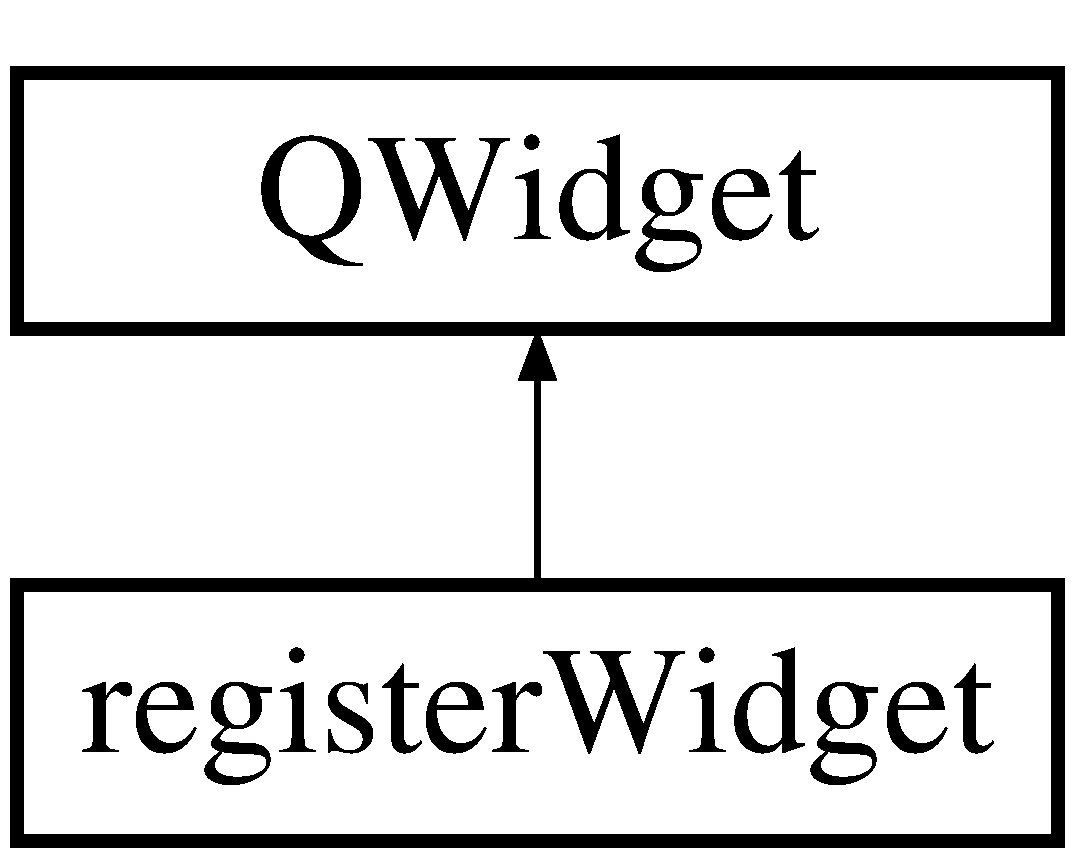
\includegraphics[height=2.000000cm]{classregisterWidget}
\end{center}
\end{figure}
\subsection*{Public Slots}
\begin{DoxyCompactItemize}
\item 
void \hyperlink{classregisterWidget_a69c2a6929e0adbd79b215812cb7c582f}{select\-Picture} ()
\begin{DoxyCompactList}\small\item\em \hyperlink{classregisterWidget_a69c2a6929e0adbd79b215812cb7c582f}{register\-Widget\-::select\-Picture} \end{DoxyCompactList}\item 
void \hyperlink{classregisterWidget_a571a61e4b370f821cc5521cca9be9747}{cancel\-Registration} ()
\begin{DoxyCompactList}\small\item\em \hyperlink{classregisterWidget_a571a61e4b370f821cc5521cca9be9747}{register\-Widget\-::cancel\-Registration} \end{DoxyCompactList}\item 
void \hyperlink{classregisterWidget_a4ffafb671340ca427f83fc2e8786f1ab}{confirm\-Registration} ()
\begin{DoxyCompactList}\small\item\em \hyperlink{classregisterWidget_a4ffafb671340ca427f83fc2e8786f1ab}{register\-Widget\-::confirm\-Registration} \end{DoxyCompactList}\item 
void \hyperlink{classregisterWidget_a80831e38d1681a00ac77e43b6f044589}{check\-Conditions} ()
\begin{DoxyCompactList}\small\item\em \hyperlink{classregisterWidget_a80831e38d1681a00ac77e43b6f044589}{register\-Widget\-::check\-Conditions} \end{DoxyCompactList}\item 
bool \hyperlink{classregisterWidget_ab26d894be588c87a21f61b45674b4a43}{pass\-Check} ()
\begin{DoxyCompactList}\small\item\em \hyperlink{classregisterWidget_ab26d894be588c87a21f61b45674b4a43}{register\-Widget\-::pass\-Check} \end{DoxyCompactList}\end{DoxyCompactItemize}
\subsection*{Public Member Functions}
\begin{DoxyCompactItemize}
\item 
\hypertarget{classregisterWidget_af5e6d9d69ab0118435e4d3f4bc5eb64d}{{\bfseries register\-Widget} (Q\-Widget $\ast$parent=0)}\label{classregisterWidget_af5e6d9d69ab0118435e4d3f4bc5eb64d}

\end{DoxyCompactItemize}
\subsection*{Public Attributes}
\begin{DoxyCompactItemize}
\item 
\hypertarget{classregisterWidget_a66a788d7d8b9b254ffc2bfe421065458}{bool \hyperlink{classregisterWidget_a66a788d7d8b9b254ffc2bfe421065458}{is\-Selected}}\label{classregisterWidget_a66a788d7d8b9b254ffc2bfe421065458}

\begin{DoxyCompactList}\small\item\em bool associated to profile picture selected \end{DoxyCompactList}\item 
\hypertarget{classregisterWidget_a782907f08a369c112237019412c93491}{Q\-Label $\ast$ \hyperlink{classregisterWidget_a782907f08a369c112237019412c93491}{welcome}}\label{classregisterWidget_a782907f08a369c112237019412c93491}

\begin{DoxyCompactList}\small\item\em text label \end{DoxyCompactList}\item 
\hypertarget{classregisterWidget_a264fd2aa96e8ba38420c793c8b4ae7e5}{Q\-Label $\ast$ \hyperlink{classregisterWidget_a264fd2aa96e8ba38420c793c8b4ae7e5}{fname}}\label{classregisterWidget_a264fd2aa96e8ba38420c793c8b4ae7e5}

\begin{DoxyCompactList}\small\item\em text label \end{DoxyCompactList}\item 
\hypertarget{classregisterWidget_a2fbf9a6aad9e9f6da6094c56e4e76719}{Q\-Line\-Edit $\ast$ \hyperlink{classregisterWidget_a2fbf9a6aad9e9f6da6094c56e4e76719}{fname\-\_\-edit}}\label{classregisterWidget_a2fbf9a6aad9e9f6da6094c56e4e76719}

\begin{DoxyCompactList}\small\item\em personal info input (fname) \end{DoxyCompactList}\item 
\hypertarget{classregisterWidget_a1ee4627bc318ca67cb4e20c96838d1b1}{Q\-Label $\ast$ \hyperlink{classregisterWidget_a1ee4627bc318ca67cb4e20c96838d1b1}{lname}}\label{classregisterWidget_a1ee4627bc318ca67cb4e20c96838d1b1}

\begin{DoxyCompactList}\small\item\em text label \end{DoxyCompactList}\item 
\hypertarget{classregisterWidget_a642e70ee1b82965daf6297788ce3e7f2}{Q\-Line\-Edit $\ast$ \hyperlink{classregisterWidget_a642e70ee1b82965daf6297788ce3e7f2}{lname\-\_\-edit}}\label{classregisterWidget_a642e70ee1b82965daf6297788ce3e7f2}

\begin{DoxyCompactList}\small\item\em personal info input (lname) \end{DoxyCompactList}\item 
\hypertarget{classregisterWidget_a50ca3c429f02b876e9649791270ce1e8}{Q\-Label $\ast$ \hyperlink{classregisterWidget_a50ca3c429f02b876e9649791270ce1e8}{username}}\label{classregisterWidget_a50ca3c429f02b876e9649791270ce1e8}

\begin{DoxyCompactList}\small\item\em text label \end{DoxyCompactList}\item 
\hypertarget{classregisterWidget_aa4ec8aad77bb7e806acedfb1ca708083}{Q\-Line\-Edit $\ast$ \hyperlink{classregisterWidget_aa4ec8aad77bb7e806acedfb1ca708083}{username\-\_\-edit}}\label{classregisterWidget_aa4ec8aad77bb7e806acedfb1ca708083}

\begin{DoxyCompactList}\small\item\em personal info input (username) \end{DoxyCompactList}\item 
\hypertarget{classregisterWidget_ab26dc88a111f294d1fb14c0ddc0d8b57}{Q\-Label $\ast$ \hyperlink{classregisterWidget_ab26dc88a111f294d1fb14c0ddc0d8b57}{password}}\label{classregisterWidget_ab26dc88a111f294d1fb14c0ddc0d8b57}

\begin{DoxyCompactList}\small\item\em text label \end{DoxyCompactList}\item 
\hypertarget{classregisterWidget_afa5e82d3c92302cd3f9c1fcc95629363}{Q\-Line\-Edit $\ast$ \hyperlink{classregisterWidget_afa5e82d3c92302cd3f9c1fcc95629363}{password\-\_\-edit}}\label{classregisterWidget_afa5e82d3c92302cd3f9c1fcc95629363}

\begin{DoxyCompactList}\small\item\em personal info input (password) \end{DoxyCompactList}\item 
\hypertarget{classregisterWidget_a84d7ea56e0c02371d10206f96b0a81b5}{Q\-Label $\ast$ \hyperlink{classregisterWidget_a84d7ea56e0c02371d10206f96b0a81b5}{passwordconf}}\label{classregisterWidget_a84d7ea56e0c02371d10206f96b0a81b5}

\begin{DoxyCompactList}\small\item\em text label \end{DoxyCompactList}\item 
\hypertarget{classregisterWidget_aeccfa539febf2a2363e9d21f21cc852e}{Q\-Line\-Edit $\ast$ \hyperlink{classregisterWidget_aeccfa539febf2a2363e9d21f21cc852e}{passwordconf\-\_\-edit}}\label{classregisterWidget_aeccfa539febf2a2363e9d21f21cc852e}

\begin{DoxyCompactList}\small\item\em personal info input (password confirmation) \end{DoxyCompactList}\item 
\hypertarget{classregisterWidget_a2a0c028a52f28ed9e62c4bdeffeb08f2}{Q\-Label $\ast$ \hyperlink{classregisterWidget_a2a0c028a52f28ed9e62c4bdeffeb08f2}{date\-\_\-text}}\label{classregisterWidget_a2a0c028a52f28ed9e62c4bdeffeb08f2}

\begin{DoxyCompactList}\small\item\em text label \end{DoxyCompactList}\item 
\hypertarget{classregisterWidget_ade5ab97f7eeaf1d52d72065e0150245f}{Q\-Date\-Edit $\ast$ \hyperlink{classregisterWidget_ade5ab97f7eeaf1d52d72065e0150245f}{date\-\_\-picker}}\label{classregisterWidget_ade5ab97f7eeaf1d52d72065e0150245f}

\begin{DoxyCompactList}\small\item\em personal info input (date picker) \end{DoxyCompactList}\item 
\hypertarget{classregisterWidget_aeb47a06757788734f8f137154bd08d1c}{Q\-Label $\ast$ \hyperlink{classregisterWidget_aeb47a06757788734f8f137154bd08d1c}{error\-\_\-message}}\label{classregisterWidget_aeb47a06757788734f8f137154bd08d1c}

\begin{DoxyCompactList}\small\item\em text label \end{DoxyCompactList}\item 
\hypertarget{classregisterWidget_adcfc9870a31cd3ec9959515219989000}{Q\-Label $\ast$ \hyperlink{classregisterWidget_adcfc9870a31cd3ec9959515219989000}{gender\-\_\-text}}\label{classregisterWidget_adcfc9870a31cd3ec9959515219989000}

\begin{DoxyCompactList}\small\item\em text label \end{DoxyCompactList}\item 
\hypertarget{classregisterWidget_a967e1a2e24940191b212756c2eedadd5}{Q\-V\-Box\-Layout $\ast$ \hyperlink{classregisterWidget_a967e1a2e24940191b212756c2eedadd5}{gender\-\_\-radio}}\label{classregisterWidget_a967e1a2e24940191b212756c2eedadd5}

\begin{DoxyCompactList}\small\item\em Layout element. \end{DoxyCompactList}\item 
\hypertarget{classregisterWidget_a2267fee33b2a5a32a5701ac963426d67}{Q\-Group\-Box $\ast$ \hyperlink{classregisterWidget_a2267fee33b2a5a32a5701ac963426d67}{gender\-\_\-container}}\label{classregisterWidget_a2267fee33b2a5a32a5701ac963426d67}

\begin{DoxyCompactList}\small\item\em Layout element. \end{DoxyCompactList}\item 
\hypertarget{classregisterWidget_af2888165eff86fc524e2e881ae0913b6}{Q\-Radio\-Button $\ast$ \hyperlink{classregisterWidget_af2888165eff86fc524e2e881ae0913b6}{male\-\_\-button}}\label{classregisterWidget_af2888165eff86fc524e2e881ae0913b6}

\begin{DoxyCompactList}\small\item\em Radio button. \end{DoxyCompactList}\item 
\hypertarget{classregisterWidget_ad58e4f850cf0208c273287fa5a7169e8}{Q\-Radio\-Button $\ast$ \hyperlink{classregisterWidget_ad58e4f850cf0208c273287fa5a7169e8}{female\-\_\-button}}\label{classregisterWidget_ad58e4f850cf0208c273287fa5a7169e8}

\begin{DoxyCompactList}\small\item\em Radio button. \end{DoxyCompactList}\item 
\hypertarget{classregisterWidget_a38c03774cddc73e3d896866f7da61cf7}{Q\-Label $\ast$ \hyperlink{classregisterWidget_a38c03774cddc73e3d896866f7da61cf7}{pppicture\-\_\-text}}\label{classregisterWidget_a38c03774cddc73e3d896866f7da61cf7}

\begin{DoxyCompactList}\small\item\em text label \end{DoxyCompactList}\item 
\hypertarget{classregisterWidget_a4cb9ac48cf6ad4136bd953e8479a74c2}{Q\-Push\-Button $\ast$ \hyperlink{classregisterWidget_a4cb9ac48cf6ad4136bd953e8479a74c2}{add\-\_\-pppicture}}\label{classregisterWidget_a4cb9ac48cf6ad4136bd953e8479a74c2}

\begin{DoxyCompactList}\small\item\em Button to open prompt to add picture. \end{DoxyCompactList}\item 
\hypertarget{classregisterWidget_a7aebfab8b880f9e7af34096679a037ee}{Q\-Label $\ast$ \hyperlink{classregisterWidget_a7aebfab8b880f9e7af34096679a037ee}{pppicture}}\label{classregisterWidget_a7aebfab8b880f9e7af34096679a037ee}

\begin{DoxyCompactList}\small\item\em Picture display. \end{DoxyCompactList}\item 
\hypertarget{classregisterWidget_a3642d8e5b279b0bbebe27dc4123c045a}{Q\-Push\-Button $\ast$ \hyperlink{classregisterWidget_a3642d8e5b279b0bbebe27dc4123c045a}{cancel}}\label{classregisterWidget_a3642d8e5b279b0bbebe27dc4123c045a}

\begin{DoxyCompactList}\small\item\em Cancel button. \end{DoxyCompactList}\item 
\hypertarget{classregisterWidget_ad4ad3b5631639eb7f47dc82853f56bc8}{Q\-Push\-Button $\ast$ \hyperlink{classregisterWidget_ad4ad3b5631639eb7f47dc82853f56bc8}{confirm}}\label{classregisterWidget_ad4ad3b5631639eb7f47dc82853f56bc8}

\begin{DoxyCompactList}\small\item\em Confirm button. \end{DoxyCompactList}\item 
\hypertarget{classregisterWidget_aa10ee76c7b26e5aadef01ab72a4b0c79}{Q\-String $\ast$ \hyperlink{classregisterWidget_aa10ee76c7b26e5aadef01ab72a4b0c79}{filename}}\label{classregisterWidget_aa10ee76c7b26e5aadef01ab72a4b0c79}

\begin{DoxyCompactList}\small\item\em Selected profile picture path. \end{DoxyCompactList}\item 
\hypertarget{classregisterWidget_a9e25b3b015d4a4fed065f626c5f16998}{Q\-File $\ast$ \hyperlink{classregisterWidget_a9e25b3b015d4a4fed065f626c5f16998}{tempfile}}\label{classregisterWidget_a9e25b3b015d4a4fed065f626c5f16998}

\begin{DoxyCompactList}\small\item\em Loaded profile picture. \end{DoxyCompactList}\item 
\hypertarget{classregisterWidget_a37756ecbb49dd1bc403707abc6a3f8de}{Q\-Grid\-Layout $\ast$ \hyperlink{classregisterWidget_a37756ecbb49dd1bc403707abc6a3f8de}{register\-\_\-layout}}\label{classregisterWidget_a37756ecbb49dd1bc403707abc6a3f8de}

\begin{DoxyCompactList}\small\item\em Main layout. \end{DoxyCompactList}\end{DoxyCompactItemize}


\subsection{Member Function Documentation}
\hypertarget{classregisterWidget_a571a61e4b370f821cc5521cca9be9747}{\index{register\-Widget@{register\-Widget}!cancel\-Registration@{cancel\-Registration}}
\index{cancel\-Registration@{cancel\-Registration}!registerWidget@{register\-Widget}}
\subsubsection[{cancel\-Registration}]{\setlength{\rightskip}{0pt plus 5cm}void register\-Widget\-::cancel\-Registration (
\begin{DoxyParamCaption}
{}
\end{DoxyParamCaption}
)\hspace{0.3cm}{\ttfamily [slot]}}}\label{classregisterWidget_a571a61e4b370f821cc5521cca9be9747}


\hyperlink{classregisterWidget_a571a61e4b370f821cc5521cca9be9747}{register\-Widget\-::cancel\-Registration} 

Cancel user registration and go back to login screen \hypertarget{classregisterWidget_a80831e38d1681a00ac77e43b6f044589}{\index{register\-Widget@{register\-Widget}!check\-Conditions@{check\-Conditions}}
\index{check\-Conditions@{check\-Conditions}!registerWidget@{register\-Widget}}
\subsubsection[{check\-Conditions}]{\setlength{\rightskip}{0pt plus 5cm}void register\-Widget\-::check\-Conditions (
\begin{DoxyParamCaption}
{}
\end{DoxyParamCaption}
)\hspace{0.3cm}{\ttfamily [slot]}}}\label{classregisterWidget_a80831e38d1681a00ac77e43b6f044589}


\hyperlink{classregisterWidget_a80831e38d1681a00ac77e43b6f044589}{register\-Widget\-::check\-Conditions} 

Check if all entries are filled and respect the criterias \hypertarget{classregisterWidget_a4ffafb671340ca427f83fc2e8786f1ab}{\index{register\-Widget@{register\-Widget}!confirm\-Registration@{confirm\-Registration}}
\index{confirm\-Registration@{confirm\-Registration}!registerWidget@{register\-Widget}}
\subsubsection[{confirm\-Registration}]{\setlength{\rightskip}{0pt plus 5cm}void register\-Widget\-::confirm\-Registration (
\begin{DoxyParamCaption}
{}
\end{DoxyParamCaption}
)\hspace{0.3cm}{\ttfamily [slot]}}}\label{classregisterWidget_a4ffafb671340ca427f83fc2e8786f1ab}


\hyperlink{classregisterWidget_a4ffafb671340ca427f83fc2e8786f1ab}{register\-Widget\-::confirm\-Registration} 

Confirm user registration and go back to login menu \hypertarget{classregisterWidget_ab26d894be588c87a21f61b45674b4a43}{\index{register\-Widget@{register\-Widget}!pass\-Check@{pass\-Check}}
\index{pass\-Check@{pass\-Check}!registerWidget@{register\-Widget}}
\subsubsection[{pass\-Check}]{\setlength{\rightskip}{0pt plus 5cm}bool register\-Widget\-::pass\-Check (
\begin{DoxyParamCaption}
{}
\end{DoxyParamCaption}
)\hspace{0.3cm}{\ttfamily [slot]}}}\label{classregisterWidget_ab26d894be588c87a21f61b45674b4a43}


\hyperlink{classregisterWidget_ab26d894be588c87a21f61b45674b4a43}{register\-Widget\-::pass\-Check} 

\begin{DoxyReturn}{Returns}
Returns whether the password follows the criterias and matches the confirmation password 
\end{DoxyReturn}
\hypertarget{classregisterWidget_a69c2a6929e0adbd79b215812cb7c582f}{\index{register\-Widget@{register\-Widget}!select\-Picture@{select\-Picture}}
\index{select\-Picture@{select\-Picture}!registerWidget@{register\-Widget}}
\subsubsection[{select\-Picture}]{\setlength{\rightskip}{0pt plus 5cm}void register\-Widget\-::select\-Picture (
\begin{DoxyParamCaption}
{}
\end{DoxyParamCaption}
)\hspace{0.3cm}{\ttfamily [slot]}}}\label{classregisterWidget_a69c2a6929e0adbd79b215812cb7c582f}


\hyperlink{classregisterWidget_a69c2a6929e0adbd79b215812cb7c582f}{register\-Widget\-::select\-Picture} 

Open prompt to let the user select a profile picture 

The documentation for this class was generated from the following files\-:\begin{DoxyCompactItemize}
\item 
registerwidget.\-h\item 
\hyperlink{registerwidget_8cpp}{registerwidget.\-cpp}\end{DoxyCompactItemize}

\chapter{File Documentation}
\hypertarget{birthdaywidget_8cpp}{\section{birthdaywidget.\-cpp File Reference}
\label{birthdaywidget_8cpp}\index{birthdaywidget.\-cpp@{birthdaywidget.\-cpp}}
}


Contains birthdaywidget class definition.  


{\ttfamily \#include \char`\"{}birthdaywidget.\-h\char`\"{}}\\*


\subsection{Detailed Description}
Contains birthdaywidget class definition. This Q\-Widget is shown whenever the user logs-\/in on his birthdate. 
\hypertarget{birthdaywidget_8h}{\section{birthdaywidget.\-h File Reference}
\label{birthdaywidget_8h}\index{birthdaywidget.\-h@{birthdaywidget.\-h}}
}


The birthdaywidget class.  


{\ttfamily \#include $<$Q\-Widget$>$}\\*
{\ttfamily \#include $<$Qt\-Widgets$>$}\\*
\subsection*{Classes}
\begin{DoxyCompactItemize}
\item 
class \hyperlink{classbirthdaywidget}{birthdaywidget}
\end{DoxyCompactItemize}


\subsection{Detailed Description}
The birthdaywidget class. 
\hypertarget{gamescene__1_8h}{\section{gamescene\-\_\-1.\-h File Reference}
\label{gamescene__1_8h}\index{gamescene\-\_\-1.\-h@{gamescene\-\_\-1.\-h}}
}


The \hyperlink{classgameScene__1}{game\-Scene\-\_\-1} class.  


{\ttfamily \#include \char`\"{}gamescene\-\_\-1\-\_\-player.\-h\char`\"{}}\\*
{\ttfamily \#include \char`\"{}gamescene\-\_\-1\-\_\-dice.\-h\char`\"{}}\\*
{\ttfamily \#include \char`\"{}gamescene\-\_\-1\-\_\-ladder\-Snake.\-h\char`\"{}}\\*
{\ttfamily \#include $<$Q\-Graphics\-Scene$>$}\\*
{\ttfamily \#include $<$Q\-Widget$>$}\\*
{\ttfamily \#include $<$Qt\-Widgets$>$}\\*
{\ttfamily \#include $<$Q\-Sound$>$}\\*
{\ttfamily \#include $<$Q\-Future$>$}\\*
{\ttfamily \#include $<$Q\-Thread$>$}\\*
{\ttfamily \#include $<$Qt\-Concurrent/\-Qt\-Concurrent$>$}\\*
{\ttfamily \#include $<$stdlib.\-h$>$}\\*
{\ttfamily \#include $<$time.\-h$>$}\\*
\subsection*{Classes}
\begin{DoxyCompactItemize}
\item 
class \hyperlink{classgameScene__1}{game\-Scene\-\_\-1}
\end{DoxyCompactItemize}


\subsection{Detailed Description}
The \hyperlink{classgameScene__1}{game\-Scene\-\_\-1} class. 
\hypertarget{gamescene__1__dice_8h}{\section{gamescene\-\_\-1\-\_\-dice.\-h File Reference}
\label{gamescene__1__dice_8h}\index{gamescene\-\_\-1\-\_\-dice.\-h@{gamescene\-\_\-1\-\_\-dice.\-h}}
}


The \hyperlink{classgameScene__1__dice}{game\-Scene\-\_\-1\-\_\-dice} class.  


{\ttfamily \#include $<$Q\-Object$>$}\\*
{\ttfamily \#include $<$Q\-Graphics\-Pixmap\-Item$>$}\\*
{\ttfamily \#include $<$Q\-Graphics\-Scene$>$}\\*
{\ttfamily \#include $<$Q\-Timer$>$}\\*
{\ttfamily \#include $<$stdlib.\-h$>$}\\*
{\ttfamily \#include $<$time.\-h$>$}\\*
\subsection*{Classes}
\begin{DoxyCompactItemize}
\item 
class \hyperlink{classgameScene__1__dice}{game\-Scene\-\_\-1\-\_\-dice}
\end{DoxyCompactItemize}


\subsection{Detailed Description}
The \hyperlink{classgameScene__1__dice}{game\-Scene\-\_\-1\-\_\-dice} class. 
\hypertarget{menuwidget_8cpp}{\section{menuwidget.\-cpp File Reference}
\label{menuwidget_8cpp}\index{menuwidget.\-cpp@{menuwidget.\-cpp}}
}


Contains \hyperlink{classmenuWidget}{menu\-Widget} class definition.  


{\ttfamily \#include \char`\"{}menuwidget.\-h\char`\"{}}\\*
{\ttfamily \#include \char`\"{}loginwidget.\-h\char`\"{}}\\*
{\ttfamily \#include \char`\"{}birthdaywidget.\-h\char`\"{}}\\*
{\ttfamily \#include \char`\"{}gamescene\-\_\-1.\-h\char`\"{}}\\*


\subsection{Detailed Description}
Contains \hyperlink{classmenuWidget}{menu\-Widget} class definition. Main menu of the application. The user can see his history, profile and access Game 1 \& Game 2 ( New game / Load Game ) 
\hypertarget{menuwidget_8h}{\section{menuwidget.\-h File Reference}
\label{menuwidget_8h}\index{menuwidget.\-h@{menuwidget.\-h}}
}


The \hyperlink{classmenuWidget}{menu\-Widget} class.  


{\ttfamily \#include $<$Q\-Widget$>$}\\*
{\ttfamily \#include $<$Qt\-Widgets$>$}\\*
\subsection*{Classes}
\begin{DoxyCompactItemize}
\item 
class \hyperlink{classmenuWidget}{menu\-Widget}
\end{DoxyCompactItemize}


\subsection{Detailed Description}
The \hyperlink{classmenuWidget}{menu\-Widget} class. 
\hypertarget{registerwidget_8cpp}{\section{registerwidget.\-cpp File Reference}
\label{registerwidget_8cpp}\index{registerwidget.\-cpp@{registerwidget.\-cpp}}
}


Contains \hyperlink{classregisterWidget}{register\-Widget} class definition.  


{\ttfamily \#include \char`\"{}registerwidget.\-h\char`\"{}}\\*
{\ttfamily \#include \char`\"{}loginwidget.\-h\char`\"{}}\\*
{\ttfamily \#include $<$Q\-Spacer\-Item$>$}\\*


\subsection{Detailed Description}
Contains \hyperlink{classregisterWidget}{register\-Widget} class definition. This page allows the user to register a new account, for use within the application 
%--- End generated contents ---

% Index
\newpage
\phantomsection
\addcontentsline{toc}{chapter}{Index}
\printindex

\end{document}
